% Development of game engine - core components & functonalities
% development of game using the game engine, including level/scene design (asset creation, scene scripting & interaction, development in general)
% UI / XP Design
% Testing & Debugging (Test cases / scenarios), (Logging, Debugger, Code Analysis), Performance Testing (-> memoization, ...), playtesting?

\chapter{Development \& Implementation}\label{ch:implementation}
In this chapter, the implementation of the game engine including the basic framework, graphic rendering and input handling is described.
The implementation of the features of the game itself are shown and the connections between different components is described by using a
UML class diagram.

\section{General Approach}\label{sec:general-approach}
The game engine was implemented as a separate, independent, enhanceable framework, which may also be used to design other
games.
It provides basic functionality for all features needed to design a game, such as input and system handling, rendering, configuration
classes and managers.
The implementation uses a basic entity-component-system as foundation and enhances this with further features.

\section{Programming Language}\label{sec:programming-language}
The programming language that was chosen for this implementation is \textit{JAVA} \\

Java is a high-level, object-oriented programming language that was originally developed by Sun Microsystems (now owned by Oracle Corporation) in the mid-1990s.
It is designed to be portable, meaning that it can be run on a wide variety of platforms, including Windows, macOS, Linux, and many others, without needing to be recompiled for each platform.
\\
Java is widely used for developing both desktop and web-based applications, as well as mobile applications for Android devices.
It is also used extensively in server-side programming and for building enterprise applications.
\\
One of the key features of Java is its virtual machine (VM), which allows Java programs to be executed on any system that has a compatible JVM installed, regardless of the underlying hardware and operating system.
This makes it possible to write a single Java program that can run on multiple platforms, without needing to be modified for each one.
\\
Java also has a large standard library of classes and functions, which makes it easier to write complex programs without needing to reinvent the wheel.
Additionally, Java is known for its strong emphasis on security, which makes it a popular choice for building applications that need to be highly secure and resistant to cyber attacks.
\\
Java was chosen because of the wide variety of standard libraries and resources available, the very object-oriented programming approach which enables for
extending and inheriting of classes to adapt objects to the games and game engines needs.
Due to garbage collection, Java enables developing without having to consider memory allocations.
Furthermore, a great benefit of using Java is the multi-platform support due to Java being an interpreted language which works
independent of operating systems or processor architectures.

\section{Game Engine}\label{sec:game}
The game engine implements a variety of methods and classes which are used for handling the general program execution, independent of the actual game implementation.
In this chapter, these classes will be explained in detail and the general concept of the engine is reviewed.

\subsection{Entity Component System}\label{subsec:entity-component-system-implementation}
The entity component system setup used in this implementation can be approached from a top-down point of view, visualized in figure \ref{fig:ecs}.
A scene is the basic class that contains all information about the currently displayed entities and the handlers and systems to be used
in the background.
There exist multiple scenes of different classes, such as scenes for the game view, menu scenes etc., which can be created by
inheriting the base scene class.
Scenes can be added to the game by using the Scene Manager, which is also used to swap between available scenes.
Each scene contains a list of entities, that could be referred to as a database of all available objects.
Entities represent a combination of different data containers, so-called components, which can be uniquely attached to each entity.
There are some standard entities and components available directly via the engine, however there may be the need for more components and entities while implementing the actual game.
The design approach of this entity component system is similar to the Unity implementation, however a few tweaks and simplifications were made in order to keep the code
simple and maintainable, while providing the changeability and flexibility of a general approach.
\begin{figure}
    \centering
    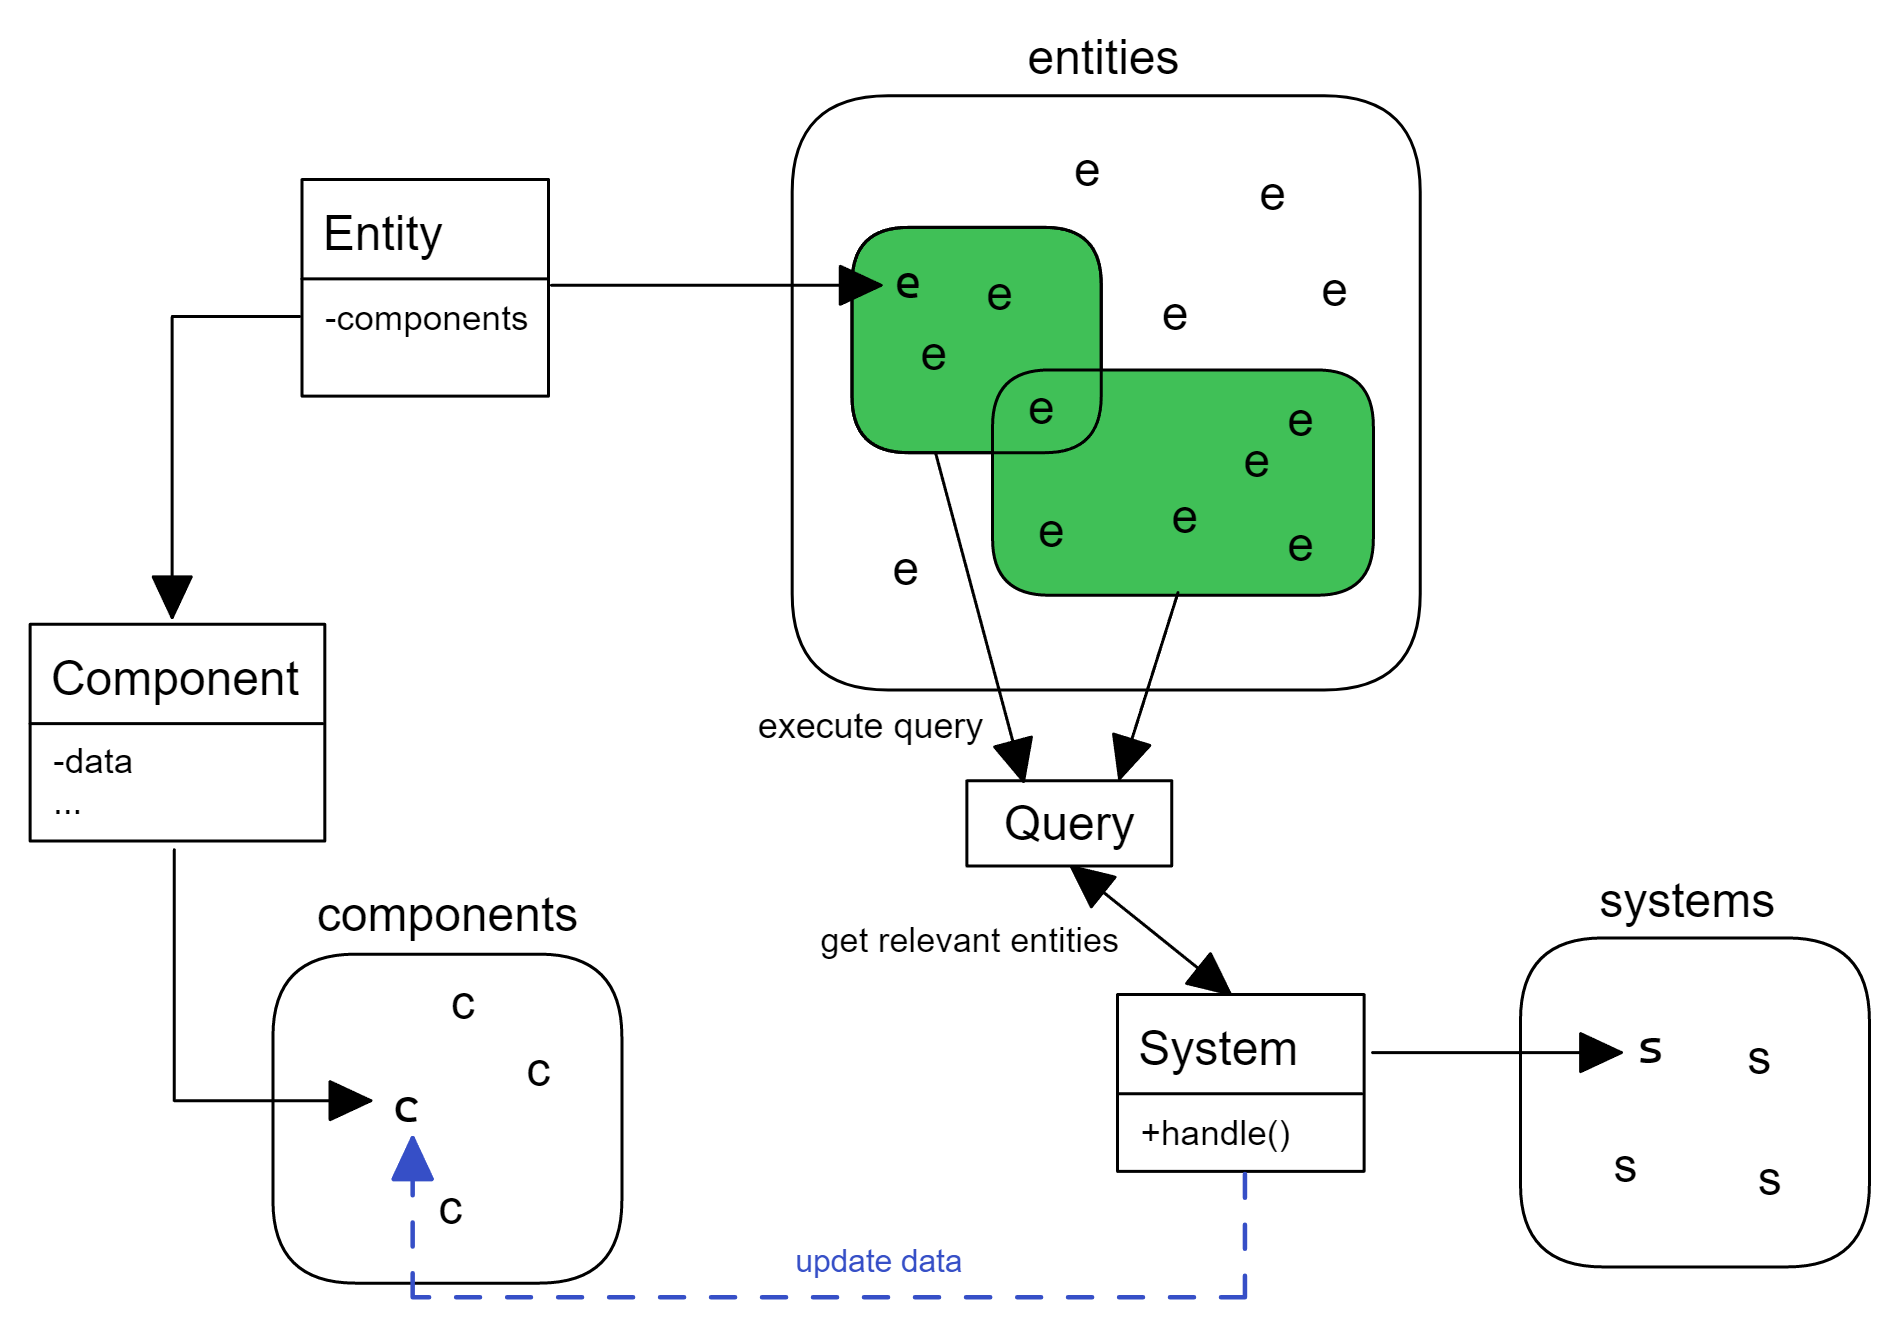
\includegraphics[width=\textwidth]{Pictures/res/implementation/ecs-database}
    \caption{ECS Database}
    \label{fig:ecs}
\end{figure}
\subsubsection{UML Diagram}\label{subsubsec:uml-diagram}
The following UML shows a simplified structure of the engine implementation, which is going to be used to explain the mechanisms
and the framework of the implementation.
\begin{figure}
    \centering
    
\includegraphics[width=1.0\textwidth]{./Pictures/res/implementation/ecs-uml}
    \caption{Simplified UML diagram of the engine implementation}
    \label{fig:ecs-block-diagram}
\end{figure}

\subsubsection{Entities}\label{subsubsec:entities}
Entities are classes constructed of different components, which could be referred to as containers storing different parameters.
Entities can not directly interact with each other, as any modification to data is strictly handled by the game engines' systems and handlers.
The Entity class implements functions to add, remove and get Components of a class type.
\\
As there are usually lots of different types of entities in a game which may contain the same components, it makes sense to inherit from the Entity class and
build generic entities which can be reused.
For GUI elements, the game engine already provides some pre-designed entities, such as buttons, text bodies, panels and image entities.
During the implementation, it was chosen to handle GUI elements as entities as well, as the game engine is purely working in 2 dimensions and therefore
rendering methods for the game itself and the GUI do not differ.
This approach was the easy choice, as having a separate class to implement UI elements would most likely end up with a lot of duplicated
code fragments, which are already implemented in the RenderingComponent, as described in the next chapter.

\subsubsection{Components}\label{subsubsec:components}
All entities are built of a subset of the available components, uniquely attached to each.
The different components will be explained in detail in the following chapter.
\\
\textbf{Render Component:} \\
The \textit{RenderComponent} class is designed to manage and store a diverse set of graphical objects that are utilized for rendering various elements within a scene.
These graphical objects are categorized into subclasses, such as text, images, animations, hovering, lines, and shapes.
Each subclass is defined by a set of parameters that dictate its appearance, including aspects like location, bounds, colors, images or animations, and text content.
\\
To address the need for rendering multiple graphical objects per entity while still adhering to the unique component-per-entity constraint, the RenderComponent class allows for the addition of each graphical object multiple times.
For example, an image that requires occasional hovering may have one object to render the image itself, and another object to render the hovering shape.
\\
Furthermore, the RenderComponent class incorporates methods that enable the retrieval of specific lists of graphical object instances based on their corresponding class.
This functionality resembles the Query implementation found in the entity component system, providing a streamlined and efficient way to access the desired graphical objects.

\textbf{ColliderComponent:} \\
Similar to the \textit{RenderComponent}, the \textit{ColliderComponent} also stores a list of collision objects, which are described by location and bounds.
Each of these collision objects is checked by the \textit{CollisionDetectionSystem} and handled accordingly, e.g.\
hovering and object at the same location as the collision object. \\ \\

\textbf{Sound Component:} \\
The \textit{SoundComponent} class can be attached to any entity that needs to have a sound played at times.
It implements methods to set the state of the sound sample to play, pause or stop and contains the actual sound sample to be used by the \textit{SoundEngine}. \\ \\

\textbf{Action Component:} \\
Action Components are used for storing a mapping of input to action within an entity, e.g.\ clicking a button which opens another scene.
Each Action Component is processed by the ActionSystem. \\ \\

\textbf{Cursor Component:} \\
The cursor component is a component used for handling game pad inputs and acts as a virtual mouse cursor, which can be moved by using
joysticks of game pads or keyboard buttons.
It simply indicates the position, where new mouse events are generated, when the actual mouse is not used. \\ \\

\subsubsection{Scene}\label{subsubsec:scene}
A scene is a collection of entities that together form an aspect of the game, e.g.\ a menu or a level.
The \textit{Scene} class is an abstract class implementing methods for adding and removing entities from itself.
The scenes in this implementation can be categorized in two general sets: menu scenes and game scenes.

\\
To add a scene to the game, a scene object needs to be instantiated and added to the games' \textit{SceneManager}, where all
scenes are stored and the currently active scene can be set.
Generally, all systems access the scene manager to only process the currently active scene, or if needed handle entities in other scenes or add / remove them.
\\

Scenes are implemented in a hierarchy which is shown in figure \todo{add figure}.

\subsubsection{Systems}\label{subsubsec:systems}
Systems are the third main part of the ECS implementation and handle any modification to the Components.
They are used for a variety of different applications and can be split into multiple sub systems, which each serve their own purpose.
The ECS implementation aims and encourages to split each function or feature into modular systems, which can then be added to the game where they are handled within the GameLoop~\ref{subsec:game-loop}.
A variety of systems is already available per default, including rendering, collision and input systems, which will be explained in the following chapters.
\\
Each system queries through the available entities / components and only processes the relevant ones.
The query system is set up as a static class that can be accessed from anywhere.
It implements methods that can be used to search for all entities of a class or entities that have a specified component
attached to it within the currently displayed scene.
The set of entities can be seen as a database that is filtered by the query system to obtain only a subset with the specified component or class type, which may be used
for other systems.
System processing is shown in figure~\ref{fig:ecs-system-processing}.
\begin{figure}
    \centering
    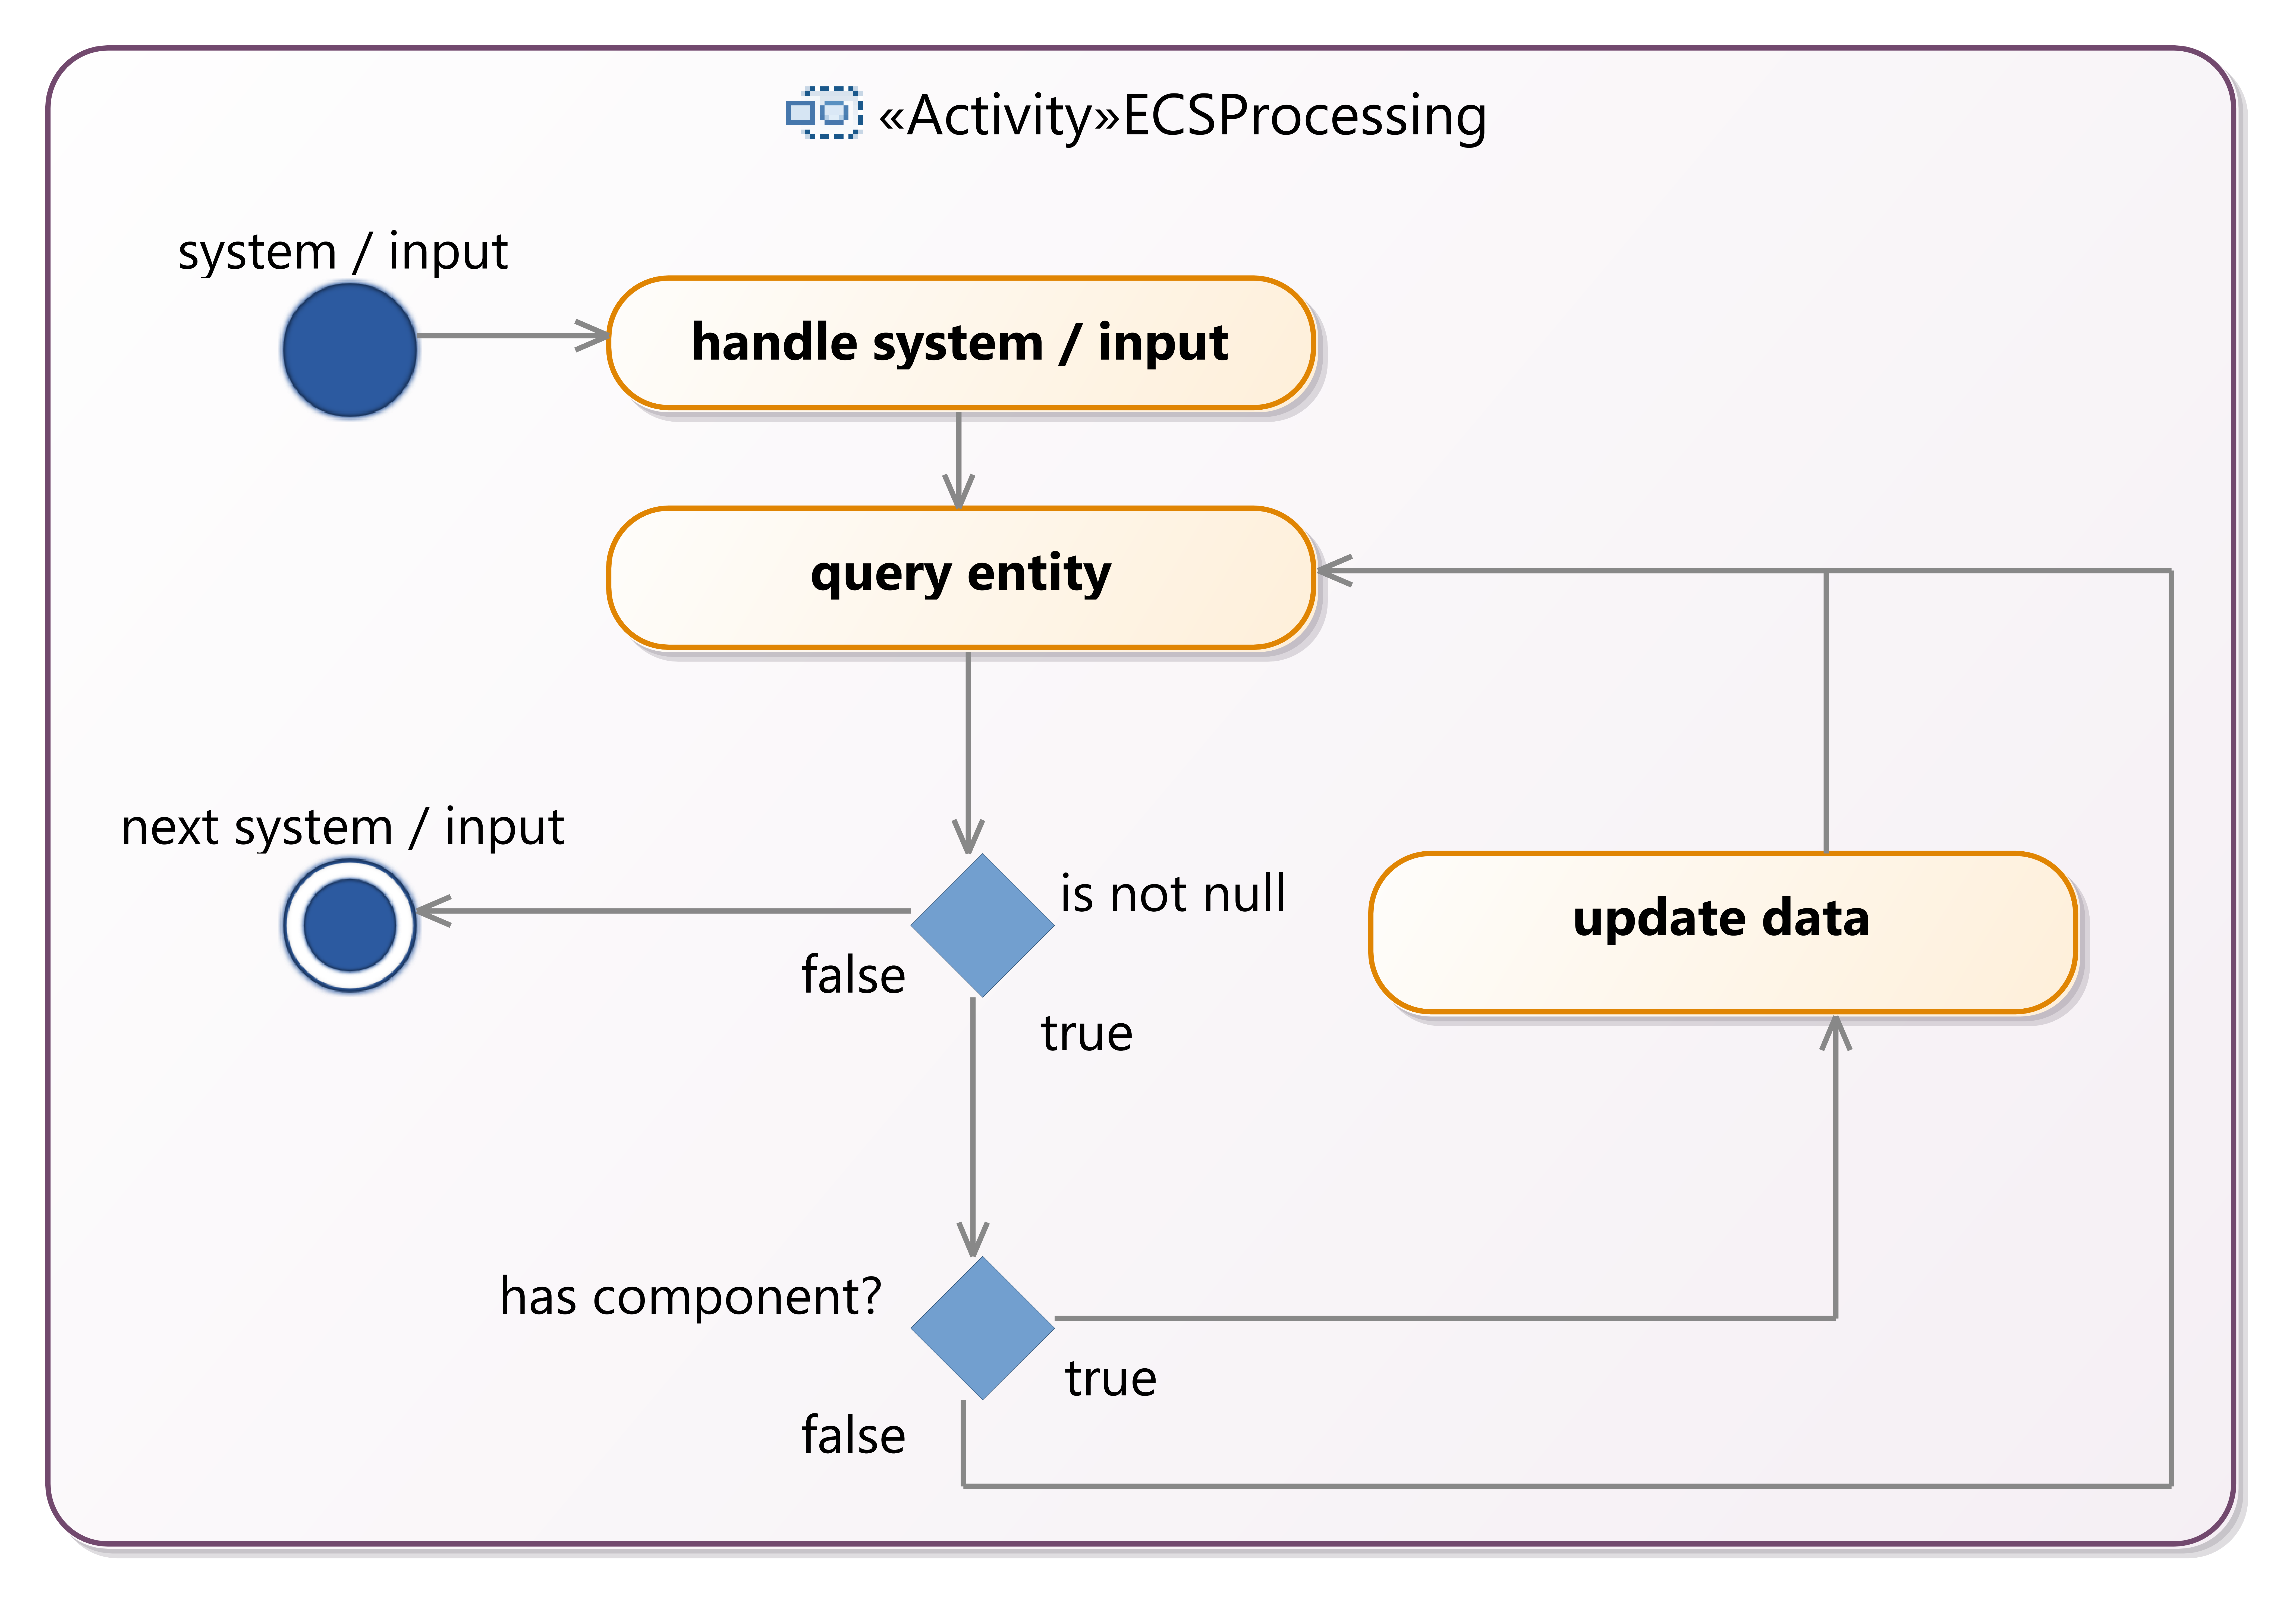
\includegraphics[width=\textwidth]{Pictures/res/implementation/ecs-system-processing}
    \caption{System processing activity diagram}
    \label{fig:ecs-system-processing}
\end{figure}
An overview of the default systems is given below.

\textbf{Action System}
Handlers are input listeners, which are event based.
They can be implemented for different purposes, such as keyboard, mouse or controller inputs in general, but also to direct inputs by the user
to a category, such as inputs for levels that trigger methods within the level itself, inputs to buttons or hovering over entities.
They provide user inputs to manipulate the systems. \todo{rewrite}

\subsection{Game Loop}\label{subsec:game-loop}
The game loop acts as the main thread of the game as soon as initialized and started.
It packs all the different systems and handlers used in the game and executes them in a given order at every time step
$t_{i} = t_{i-1} + \Delta t$, where $\Delta t$ is the execution rate defined for the game.
An exception to this order is the input recording, which is handled in a separate, synchronized thread, as described in chapter~\ref{subsec:input-recording}.
In this implementation, $\Delta t$ is defined as $\Delta t = 1000 / 240 ms = 4.1667 ms$, which equals 240 calculated frames per second that may be shown and rendered
to the screen, if available.
\\ \\
The execution order of the game loop can be seen in figure~\ref{fig:gameloop-process}.
\begin{figure}
    \centering
    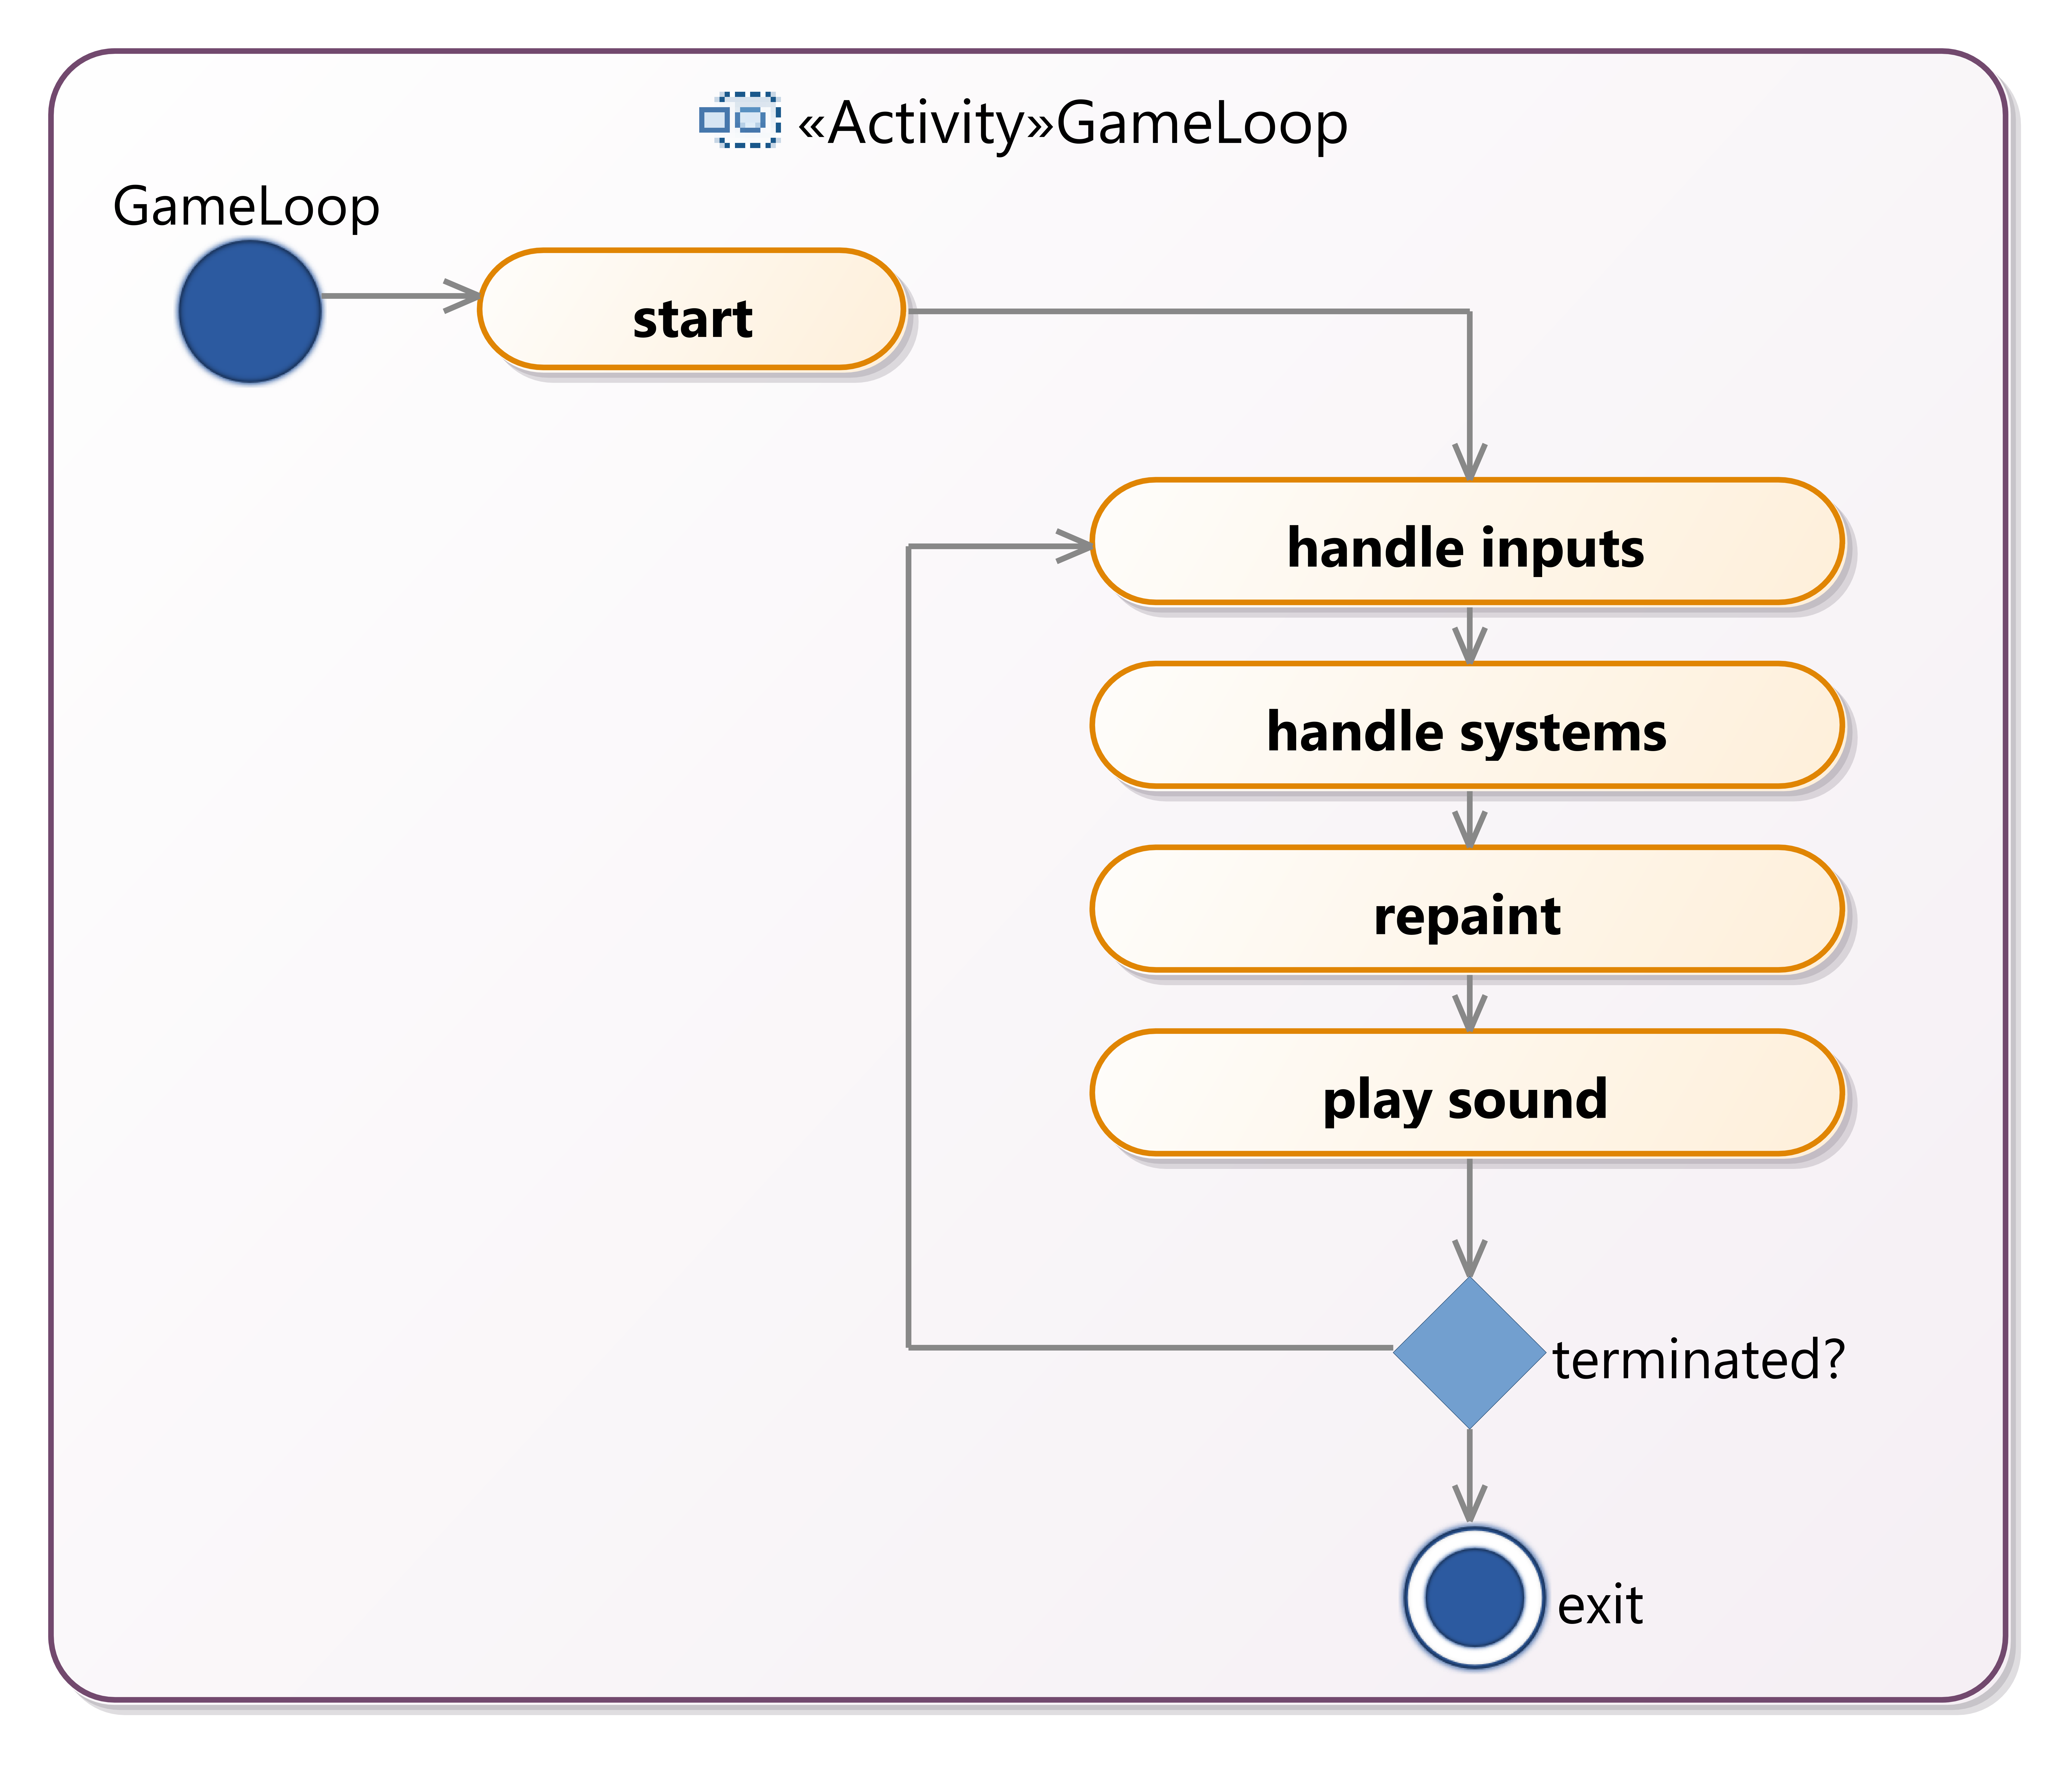
\includegraphics[width=\textwidth]{Pictures/res/implementation/gameloop-process}
    \caption{Game loop execution order}
    \label{fig:gameloop-process}
\end{figure}

\subsection{Input Recording}\label{subsec:input-recording}
Input recording is executed in a separate thread and handles inputs at a rate of $\delta t_{inputs} = 20 ms$, since inputs in between two frames
would otherwise not be received by the games' input handling system.
$20 ms$ is a delta time at which most input devices send button inputs, according to manufacturer specifications, therefore it is suitable for this application as well. \todo{add note}
\\
Generally, a button press needs to be differentiated from a button click.
While a button press is a continuous event, a button click is a one time event defined as the state change from button is not pressed to button is pressed.
Each recorded event, either from ActionListeners implemented directly on the rendering panel or from the GamePadAdapter are queued to the engines input handling system~\ref{subsec:input-handling}.
\\
The game pad integration will be explained in a later chapter~\ref{subsec:gamepad-integration}.
\subsection{Input Handling}\label{subsec:input-handling}
The InputManager contains a list of all Handlers available to the game, implements methods to add and remove objects of the Handler class and methods to queue events
to a list of events per type - Mouse Event, Key Event and Input Action (controller inputs).
\\
Each handler connected to the InputManager will receive all the events available in the respective event queues at the given time step and execute their handling methods, which
then execute the actual actions on the game and its entities.
The handler class is an abstract class that can be inherited to implement a variety of handlers, depending on the game requirements.
One specific handler class, the CollisionDetectionHandler is implemented by default and allows for an easy implementation of hovering and clicking entities with a ColliderComponent.
It checks the current mouse position (given in the latest mouse event) and handles a potential collision with an Entity.

\subsection{System Handling}\label{subsec:system-handling}
Systems are time-based and triggered with every update loop of the game.
Systems do not have specific handling methods for input types, they operate solely time-based and execute a pre-defined logic.
They contain methods for different calculations, game logic or time-based events and actions.
Again, the System class is an abstract class that can be inherited from to implemented system classes according to the game requirements.
An ActionSystem is already implemented, which is used to handle different types of actions that can be triggered e.g.\ by pressing a button entity, which starts
another scene.
The reason for this system being time based instead of event based is, that the CollisionDetectionHandler already sets the state of the Components,
however possible ActionComponents need to be handled as well.
If a CollisionObject is clicked or hovered, the ActionSystem will check for possible actions to execute available from the ActionComponent.

\subsection{Scene Update \& Repaint}\label{subsec:scene-update-&-repaint}
The next step in the game loop is a generic update of the currently active scene, which may be removing any unnecessary entities based on different conditions or
checking for a state change after an input or action has been handled.
After the update, the active scene is repainted by the RenderingEngine~\ref{subsec:graphics-engine}.

\subsection{Rendering Engine}\label{subsec:graphics-engine}
The RenderingEngine is a static class implemented within the game engine to handle all visible objects, screen rendering and scaling.
All content is rendered to a JPanel object by using the Graphics2D instance available by default, this is called the RenderingPanel.
\\
The RenderingEngine receives scaling factors for width and length from the ScalingEngine and the RenderConfiguration classes, which handle resizing the frame,
fullscreen mode and different screen resolutions as well as antialiasing options.
During the rendering cycle, every location and boundary of the RenderObjects is scaled and only afterwards it is rendered, however the original design position
is always present in the RenderObject parameters.
This is necessary to correctly handle rescaling.
\\
A rendering cycle executes a few different methods which are all called by the overwritten repaint method from the RenderingPanel.
First, all entities with a RenderComponent are queried by the Query system of the game engine and added to the rendering stack.
This stack is then split up into multiple stacks of RenderObjects, which are the objects saved to the component that describe the actual graphical visualization, based
on their rendering layer.
Each layer is rendered one after another by using specific rendering classes for different objects such as images, text or shapes.
Layering allows for stacking of multiple graphical entities above each other and allows for a better design of GUIs and the game itself.
The following layers are rendered in this order:
\begin{enumerate}
    \item Background
    \item Game Layer 1
    \item Game Layer 2
    \item Game Layer 3
    \item Game Hover Layer
    \item UI Layer 1
    \item UI Layer 2
    \item UI Hover Layer
\end{enumerate}
For example, if a simple composition of background image, game entity and UI should be rendered at the same position, the UI will always be in front of the game entity located at any of the game layers,
while the game entity will always overwrite the background at that position.
The reason for multiple UI and Game layers is simply to allow for a greater variety and range of possibilities when it comes to designing the game scenes.
\\
For better visualization, the full rendering cycle is shown in figure x~\todo{add figure}.

\subsection{Sound Engine}\label{subsec:sound-engine}
A SoundEngine is implemented in the Game Engine, which handles playing, pausing and stopping any audio stream available.
During each cycle, the SoundEngine collects all entities with a SoundComponent available, and checks if they are already playing and if not, if they should be playing.
The Java built-in library \textit{Clip} is used to play audio streams and loop them if necessary.
This allows for an easy handling of any sound that should be played during a game, e.g.\ background music or button click sounds.

\subsection{Utility Classes}\label{subsec:utility-classes}
Apart from the Game Loop, there are also multiple other configuration classes, managers, systems and utility classes, which will be explained in depth in this chapter.
\subsubsection{Game Configuration}\label{subsubsec:game-configuration}
The GameConfiguration class by default implements a random profile name chosen of a variety of different names at game start, which is then used for saving high-scores
or may also be used in other parts of the game.
It also contains parameters for the currently active language, rendering configuration and sound configuration.

\subsubsection{Game Information}\label{subsubsec:game-information}
In the GameInformation class, some generic variables for a title of the game, authors, version and description can be set, which are then used for instance as the games frame
title.

\subsubsection{Scene Manager}\label{subsubsec:scene-manager}
The SceneManager is the main storage of all scenes, which may be menu scenes such as main menus or level scenes, i.e.\ game maps.
It can be called from anywhere within the game to switch a scene to another loaded scene or add a new scene.

\subsubsection{Resource Manager}\label{subsubsec:resource-manager}
The ResourceManager is used for loading any kind of resource from outside the Java classes, e.g.\ audio files, images or xml data and processes
these resources accordingly.
There are multiple implementations which are used by the ResourceManager for loading of different XML files, such as high-scores (HighScoreManager) or languages (LanguageManager),
however the basic implementation of the ResourceManager equals their implementation and therefore the XML parsing and processing is going to be described only for the ResourceManager.
The following resource can be loaded by the resource manager and its sub manager classes:
\begin{itemize}
    \item Images, using the method \textit{loadImage()}
    \item Fonts, using the method \textit{loadFont()}
    \item
\end{itemize}
\subsubsection{Logging}\label{subsubsec:logging}
The Java logging tool is available and easily accessible from any class by simply using the static function implemented in the Game class and adding information to
the logger, which needs a specified log level and message to log.

\subsubsection{Styling \& Design}\label{subsubsec:styling-&-design}
A basic color scheme and font collection is already directly implemented to the game and can be used from scratch, without loading other fonts or having to think about
color schemes.
This allows for a quick and easy design of graphical components.

\section{Game Implementation}\label{sec:game-implementation}
This chapter focuses on the actual implementation of the game, while explaining where the generic game engine is used and why.
The different systems implemented for calculating the game mechanics are detailed.
\subsection{Handler}\label{subsec:handler}
Handlers, as already pointed out, are used to handle user inputs and trigger certain things within the game.
The implemented handlers for the game will be explained in this chapter.
\subsubsection{Build Handler}\label{subsubsec:build-handler}
The BuildHandler is used to handle the placement, replacement, removal and connection of components to the game grid.
There are different SimulationTypes, which are handled differently.
For the component and cable placement, the following constraints apply:
On each game grid tile, there may only be exactly one component of type ACTUATOR, SENSOR, COMPUTER or VOTER.
If any of the above-mentioned components exists on a tile, no cable may be placed at this position.
CABLE type components are handled differently, as there may be cables of different types (red, blue, green, yellow) on the same tile, to enable
cross strapping of different components.
Cables can be rotated at both ends to correctly connect components as wanted.
Whenever a cable or component is placed or rotated, the connections are updated.
To display this connection, cable ports are used.
Each cable port can be used to connect a single other entity to the cable port.
Sensors have 4 cable ports with the type output, respectively actuators have 4 cable ports with type input.
Computers and voters have in and out puts, whereas cables only have a single in and output.
When replacing or removing a component, the removed component will be put back to the build panel.

\subsubsection{CursorSelectorHandler}\label{subsubsec:cursorselectorhandler}
For handling game pad and keyboard inputs, the cursor selector handler was implemented.
It creates a globally available entity (meaning, it is available in every scene), which displays a virtual cursor that can be
moved around by using the keyboard arrows or the joysticks of a gamepad.
It handles all input actions coming from gamepads and key events coming from the keyboard, and converts them to their according mouse events.
In this way, all other handler implementations only need to handle mouse events, which are virtually queued from the cursor selector handler.

\subsection{System}\label{subsec:system}
\subsubsection{Simulation System}\label{subsubsec:simulation-system}
The simulation system handles updates of the current components on the game field, as well as starting the game goal
validation by using the MarkovProcessor~\ref{subsubsec:example-markov-chains}.
\\
Each cycle of the simulation systems executes four different methods.
At first, the group ids of each simulation entity are updated, as well their input ids.
This is needed in order for every entity to know to which other entities they are connected, which is necessary to correctly
update their states, both during the building mode and during the Markov simulation, where these connections are copied.
After updating the state, the graphical representation of each state is changed, depending on the actual state.
This shows, if an entity is correctly connected and working, or if it is currently not connected.
\\
The markov chain calculation is always run in a separate thread, which allows for correctly rendering the animations that occur during the calculation, i.e.\ the aircraft movement through the sky.
When the calculation of the markov chain is finished, all states that lead to a system failure taking into consideration the level
goal and requirements (minimum correctly working components, system failure probability, maximum out of control components) are
searched for and added up to calculate the system failure probability.
For both, the out of control failure and passive failure, this probability is calculated separately.
Afterwards, if the probabilities meet the level target and the validation is successful,
from the probabilities, the leftover components in the build panel and a base level score, the total score reached is calculated using the following equations.
Each level has a set base score when finishing the level.
\begin{equation}
    s_{base} = 100
    \label{eq:base-score}
\end{equation}
The probabilities of the current state calculated are compared to the target requirement failure probability by comparing the number of exponentials of 10 to each other.
\begin{equation}
    s_{accuracy} = 10 \cdot \lvert \log_{10} p(state) - \log_{10} p(goal)\rvert
    \label{eq:accuracy-score}
\end{equation}
The component score is defined as the sum of all components that are still available to the player in the build panel (excluding cables).
\begin{equation}
    s_{component} = \sum_{i = 1}^{components} 10
    \label{eq:component-score}
\end{equation}
The total score is the sum of the 3 previously calculated scores.
\begin{equation}
    s_{total} = s_{base} + s_{accuracy} + s_{components}
    \label{eq:total-score}
\end{equation}
Each score is shown separately in the score overview, with an additional indication of the accuracy of the probabilities to the target.
The user can see, where he or she may improve the system in order to get closer to the target.
This scale is also shown, when the validation of the target requirements is not passed by the currently built system, to indicate
a hint on what could be improved by the user.
\\
To correctly validate the goal, the actual probability calculated is summed up with an epsilon value of $\epsilon = 1e-7$,
to prevent incorrect validations due to rounding errors in double values.
The double precision floating point error occurs due to the internal representation, which can only represent a specified range of
values.
Therefore, especially when working with very small or very large numbers, rounding errors (i.e.\ the next representable value by the internal structure which can be stored
in the binary format) occur.
\subsubsection{Markov Processor}\label{subsubsec:example-markov-chains}
In the following chapter, some examples for Markov chains that represent the level designs will be shown and the implementation of the
MarkovProcessor will be explained by using these graphs.

\\ \\

The Markov Processor generates a markov chain, based on the given entities and available groups and inputs provided from the SimulationSystem.
First, a starting state, including all the relevant Entities is generated.
Each state is represented as a MarkovState, which contains the probability of the state occurrence and a list of MarkovStateObjects, that represent the different entities available after validating
the current level.
This step is needed in order to generate all the different MarkovStates without actually modifying the game grid.
\\ \\
For demonstration purpose, a simple system state with a single sensor, computer and actuator is used.
Whenever a failure state is update to passive or out of control, all other components will also be updated accordingly, which can also be seen in the graph~\ref{fig:markov-simplex}.
The indices used are as follows: S = Sensor, C = Computer, A = Actuator.
The failure probabilities of each component are:
\begin{equation}
    \lambda_{f,S} = 1\text{e-}4
    \label{eq:markov-1}
\end{equation}
\begin{equation}
    \lambda_{f,C} = 1\text{e-}4
    \label{eq:markov-2}
\end{equation}
\begin{equation}
    \lambda_{f,A} = 0
    \label{eq:markov-3}
\end{equation}
For the failure detection ratio, the following values are used:
\begin{equation}
    C_{S} = 0.9
    \label{eq:markov-4}
\end{equation}
\begin{equation}
    C_{C} = 0.9
    \label{eq:markov-5}
\end{equation}
\begin{equation}
    C_{A} = 1
    \label{eq:markov-6}
\end{equation}

\begin{figure}
    \begin{center}
        \scalebox{0.33}{
            \begin{tikzpicture}[->, >=stealth', semithick, node distance=7cm, auto]
            \tikzset{rectangle/.append style={draw=black, thick, fill=white}}
            \node    (S)[font=\fontsize{24}{0}\selectfont]  {\TBox[fill=white]{Sensor}};
            \node    (C)[font=\fontsize{24}{0}\selectfont, right of=S]  {\TBox[fill=white]{Computer}};
            \node    (A)[font=\fontsize{24}{0}\selectfont, right of=C]  {\TBox[fill=white]{Actuator}};
            \path
    (S) edge (C)
    (C) edge (A)
            \end{tikzpicture}
        }
    \end{center}\caption{Example System System}
    \label{fig:simplex}
\end{figure}


\begin{figure}
\begin{center}
    \scalebox{0.33}{
        \begin{tikzpicture}[->, >=stealth', semithick, node distance=7cm, auto]
        \tikzset{rectangle/.append style={draw=black, thick, fill=white}}
        \node    (A)[font=\fontsize{20}{0}\selectfont]  {\TBox[fill=white]{C}\TBox[fill=white]{C}\TBox[fill=white]{C}};
        \node    (B)[font=\fontsize{20}{0}\selectfont,below of=A]   {\TBox[fill=white]{C}\TBox[fill=white]{F}\TBox[fill=white]{C}};
        \node       (C)[font=\fontsize{20}{0}\selectfont,left of=B] {\TBox[fill=white]{F}\TBox[fill=white]{C}\TBox[fill=white]{C}};
        \node (D)[font=\fontsize{20}{0}\selectfont,right of=B] {\TBox[fill=white]{C}\TBox[fill=white]{C}\TBox[fill=white]{F}};
        \node (G)[font=\fontsize{20}{0}\selectfont,below left of=B] {\TBox[fill=white]{C}\TBox[fill=blue!30]{P}\TBox[fill=blue!30]{P}};
        \node (H)[font=\fontsize{20}{0}\selectfont,below right of=B] {\TBox[fill=white]{C}\TBox[fill=red!30]{O}\TBox[fill=red!30]{O}};
        \node (F)[font=\fontsize{20}{0}\selectfont,left of=G] {\TBox[fill=red!30]{O}\TBox[fill=red!30]{O}\TBox[fill=red!30]{O}};
        \node (E)[font=\fontsize{20}{0}\selectfont,left of=F] {\TBox[fill=blue!30]{P}\TBox[fill=blue!30]{P}\TBox[fill=blue!30]{P}};
        \node (I)[font=\fontsize{20}{0}\selectfont,right of=H] {\TBox[fill=white]{C}\TBox[fill=white]{C}\TBox[fill=blue!30]{P}};
        \node (J)[font=\fontsize{20}{0}\selectfont,right of=I] {\TBox[fill=white]{C}\TBox[fill=white]{C}\TBox[fill=red!30]{P}};
        \path
    (A) edge[font=\fontsize{20}{0}\selectfont,left,pos=0.8]     node{$\dot{p_2}=\lambda_{f,C} \cdot p_1$}     (B)
        edge[font=\fontsize{20}{0}\selectfont,above left,pos=0.2]    node{$\dot{p_3}=\lambda_{f,S} \cdot p_1$}      (C)
        edge[font=\fontsize{20}{0}\selectfont,above right,pos=0.2]    node{$\dot{p_4}=\lambda_{f,A} \cdot p_1$}      (D)
        (C) edge[font=\fontsize{20}{0}\selectfont,above left,pos=0.5] node{$p_5=\dot{p_3} \cdot C_S$} (E)
        edge[font=\fontsize{20}{0}\selectfont,below right,pos=0.6] node{$p_6=\dot{p_3} \cdot (1-C_S)$} (F)
        (B) edge[font=\fontsize{20}{0}\selectfont,above left,pos=0.4] node{$p_7=\dot{p_2} \cdot C_C$} (G)
        edge[font=\fontsize{20}{0}\selectfont,above right,pos=0.4] node{$p_8=\dot{p_2} \cdot (1-C_C)$} (H)
        (D) edge[font=\fontsize{20}{0}\selectfont,below left,pos=0.8] node{$p_9=\dot{p_4} \cdot C_A$} (I)
        edge[font=\fontsize{20}{0}\selectfont,above right,pos=0.5] node{$p_{10}=\dot{p_4} \cdot (1-C_A)$} (J)
        \end{tikzpicture}
    }
\end{center}
\caption{Markov Chain Simplex System}
\label{fig:markov-simplex}

\end{figure}
The markov chain for these parameters can be seen in figure \todo{add fig}.
\\
The implementation starts by generating a starting node, where all states are set to correct for the available components.
This state has a set probability of 1.
For each new state, the transition probability to this state from the previous state is calculated by multiplying the previous state probability with the
failure probability of the current failed component.
From there, each branch splits into two branches, one taking into consideration the failure detection ratio to calculate the passive failure state, the other for calculating the
out of control failure state.
\\
The approach of the implementation always sets the previous and the next states from a current state accordingly, so the tree-like
graph can be searched for specific states and state transitions.
Eventually, to receive the failure probability for a given state or a given set of states (e.g.\ all states that lead to a system failure), there is an algorithm
that finds exactly these states and calculates the sum of their probabilities.
Here, the failure probability for a time step of $t = 1 \text{h}$ is used, which results in a simplification of the general equations that removes all the integrations.
Therefore, only the state transition probabilities have to be summed up to calculate the actual probability for a specific set of states that can or cannot occur.
For larger or smaller time steps, instead of directly adding up the state transition probabilities, one would need to integrate the probability n times, based on the amount of nodes
/ states that are previous to each state.
\\
\\
A during the implementation was the performance optimization for markov chains with increasing amount of system components.
There were two different approaches to the implementation, which are described below.
\paragraph{Recursive Markov Chain Generation}
New MarkovStates are generated recursively, by calling the method from within the method directly after creating and adding a new state to the next state list of a Markov State.
This is calculated, until the break criteria is reached, which is, when a branch of the train is calculated until its very end, where all MarkovStateObjects are in
one of the two failed states, either OOC or PASSIVE\@.
\paragraph{Iterative Markov Chain Generation}
In the same way that states are calculated recursively, the same method was also implemented in an iterative manner,
after performance issues occurred with the recursion.
This is implemented via a stack, which is iterated through until it is empty.
With each iteration, new MarkovStates are added to the stack, until each branch is finished, i.e.\ all MarkovStateObjects are in a failed state.
\paragraph{Memoization}
To further optimize the algorithm, memoization was implemented.
Memoization is a programming technique used to optimize the execution time of computationally expensive functions by caching their results for a given set of input parameters.
When a memoized function is called with the same input parameters as a previous call, the cached result is returned instead of re-computing the function.
In the implementation, a HashMap is used, that stores each MarkovState as a key-value pair by using a hash code calculated from the current MarkovStateObjects states.
Whenever another state change would require the MarkovProcessor to calculate a state already available in this map, the MarkovState is instead cloned from there instead,
as the same MarkovState means, that the exact same components have failed.

\subsection{Scene}\label{subsec:scenes}
A hierarchical scene structure was implemented to the game, which can be seen in figure \ref{fig:scenes-hierachry}.
The base scene contains elements of the game that are visible in every scene, and therefore can be inherited to all other scene classes.
This includes the games background image and generic option buttons for settings, sound, back to menu and exit.
From this base scene, a base menu scene and a base game scene are inherited, which are used to display different menu screens and contain
the basic elements necessary to play the game or build maps in the build mode.
These scenes inherit multiple other scenes, which show different menus (main menu, level map, settings menu) and game scenes (main game scene, build mode scene, tutorial scene).
Specifically for tutorials, an interface which implements methods to display tutorials has been added to the game, which describes classes as tutorial classes.
Whenever a tutorial dialogue needs to be handled, this interface has to be implemented.

\begin{figure}
    \centering
    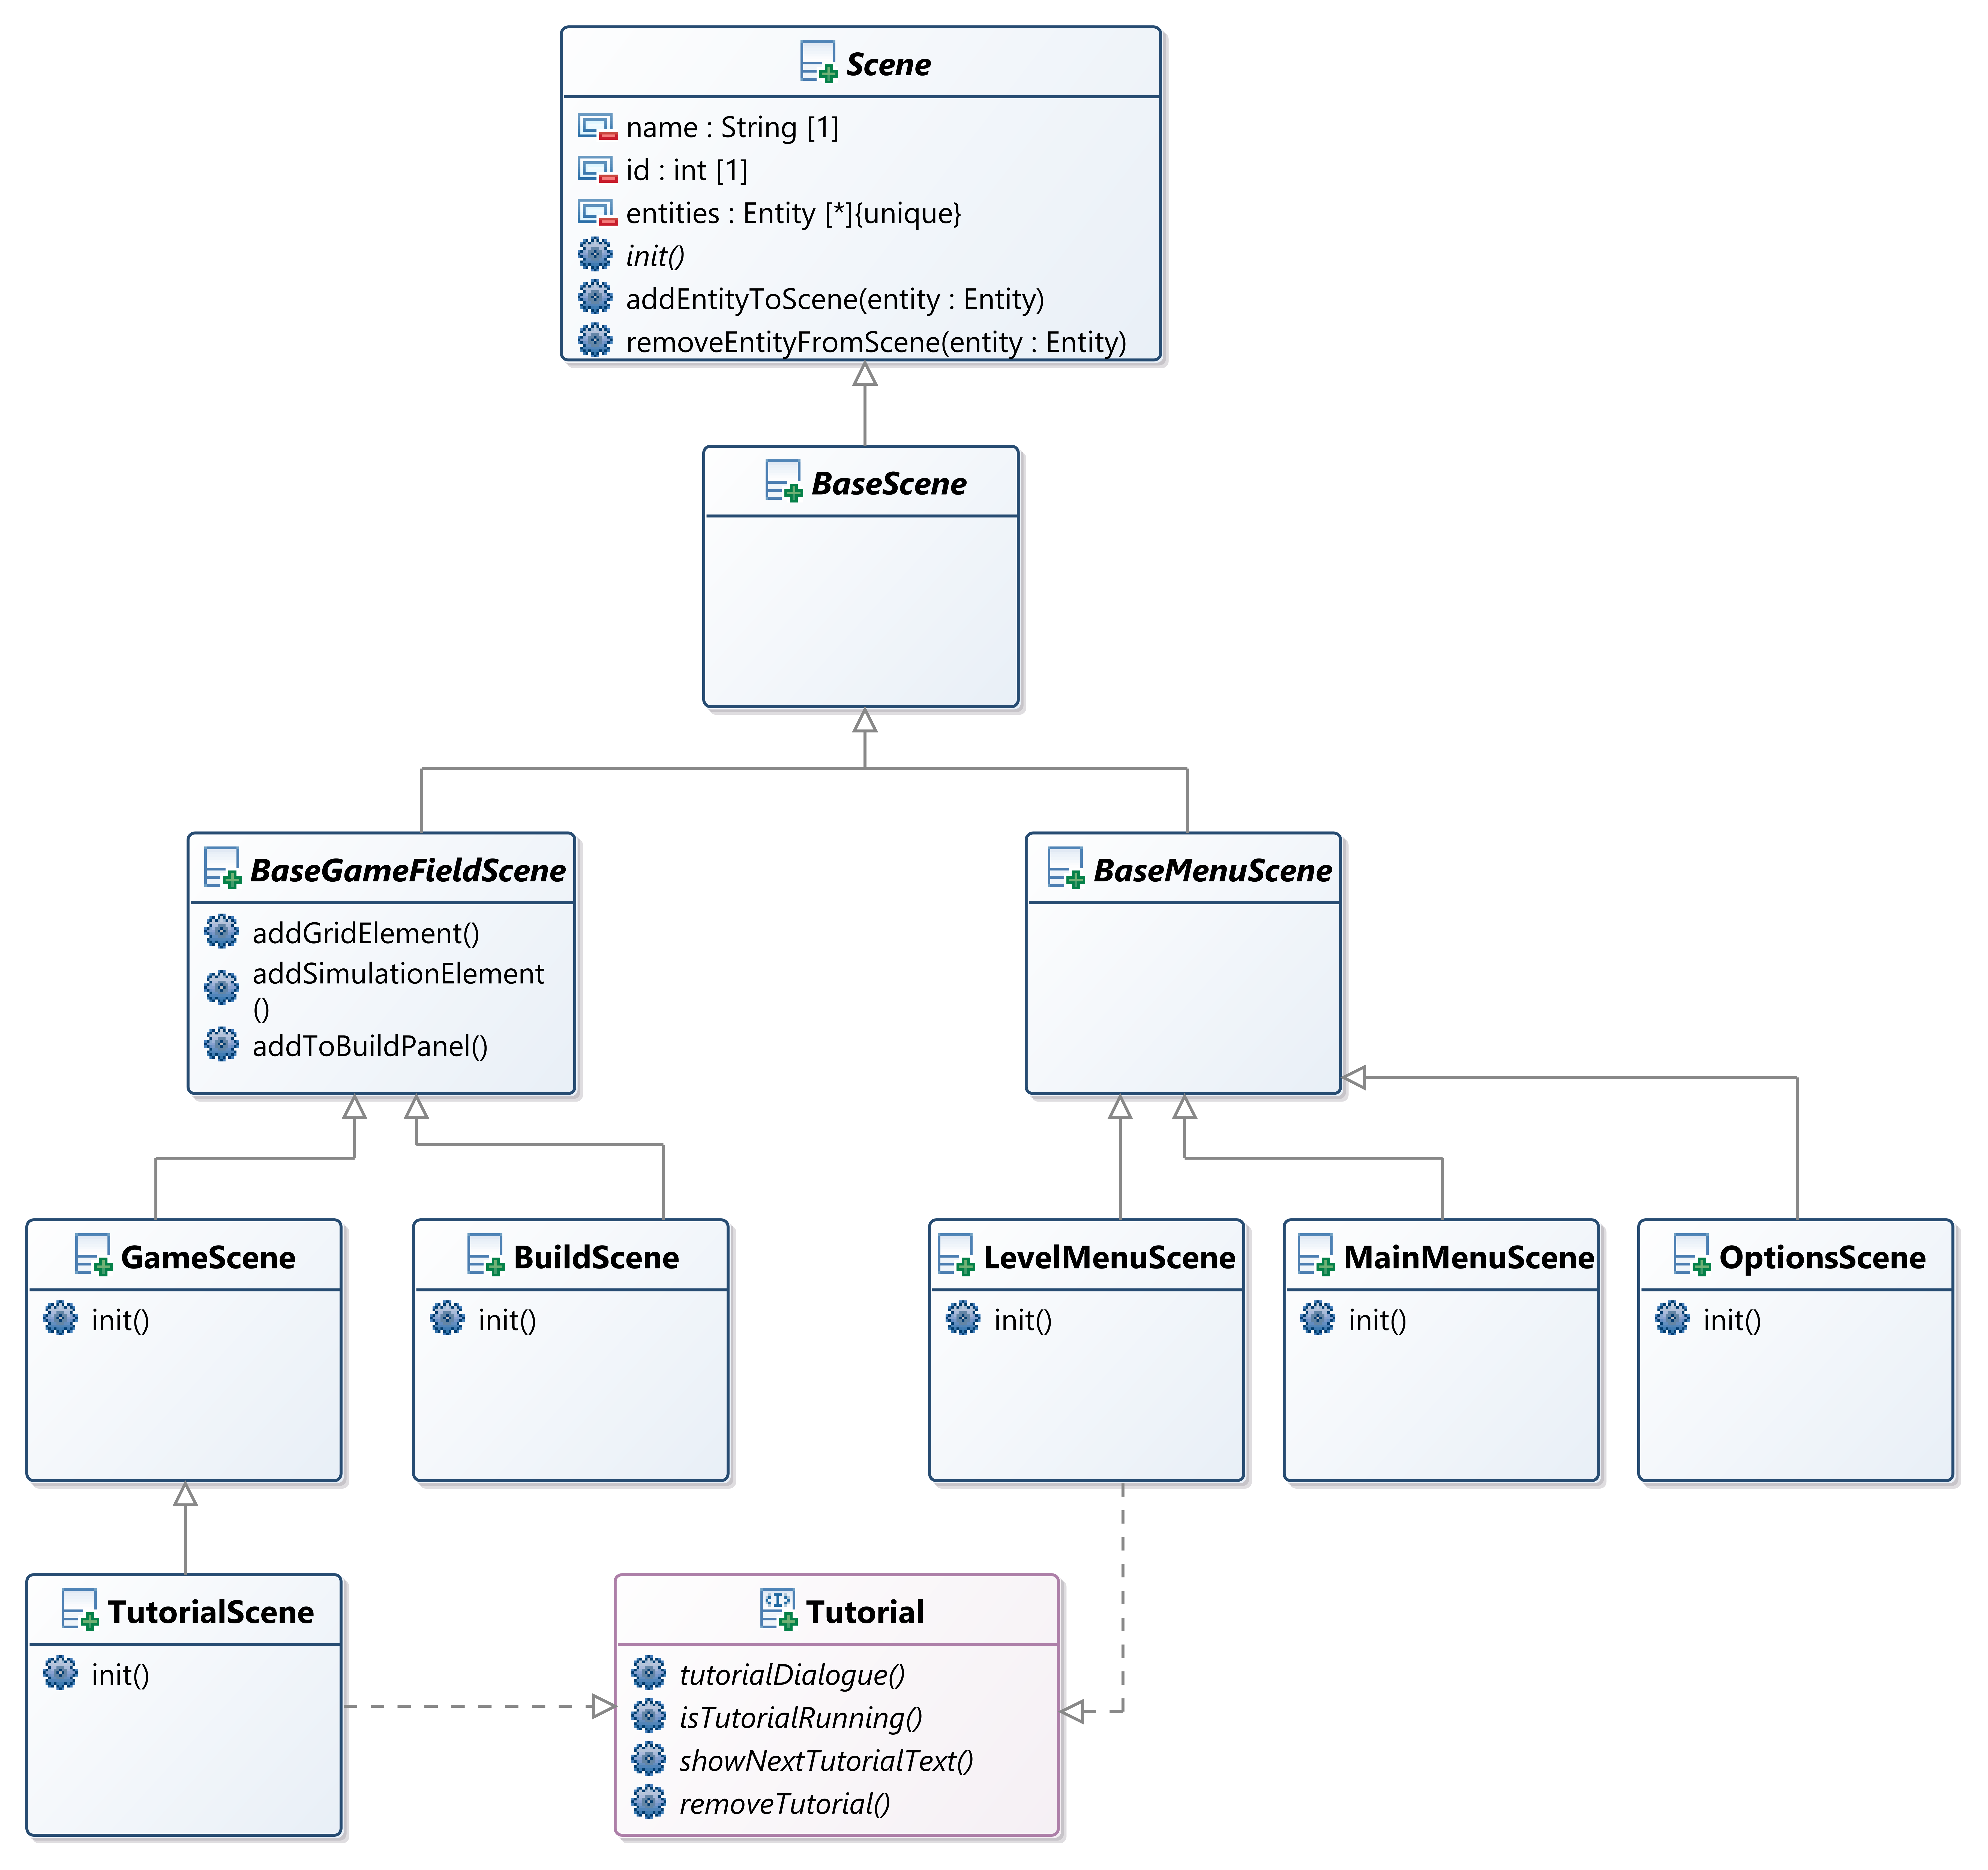
\includegraphics[width=\textwidth]{Pictures/res/implementation/scenes-hierarchy}
    \caption{Scene hierarchy}
    \label{fig:scenes-hierachry}
\end{figure}

The basic layout of the scenes was already described in~\ref{subsec:graphic-design}, the finished implementation of these
layouts is visualized in figures~\ref{fig:game-scene} and~\ref{fig:level-scene}.
Furthermore, the menu scene implementation is displayed in figure~\ref{fig:menu-scene}.
\todo{figures wirklich so?}
\begin{figure}
    \centering
    \setlength{\fboxsep}{1pt}
    \setlength{\fboxrule}{1pt}
    \fbox{
        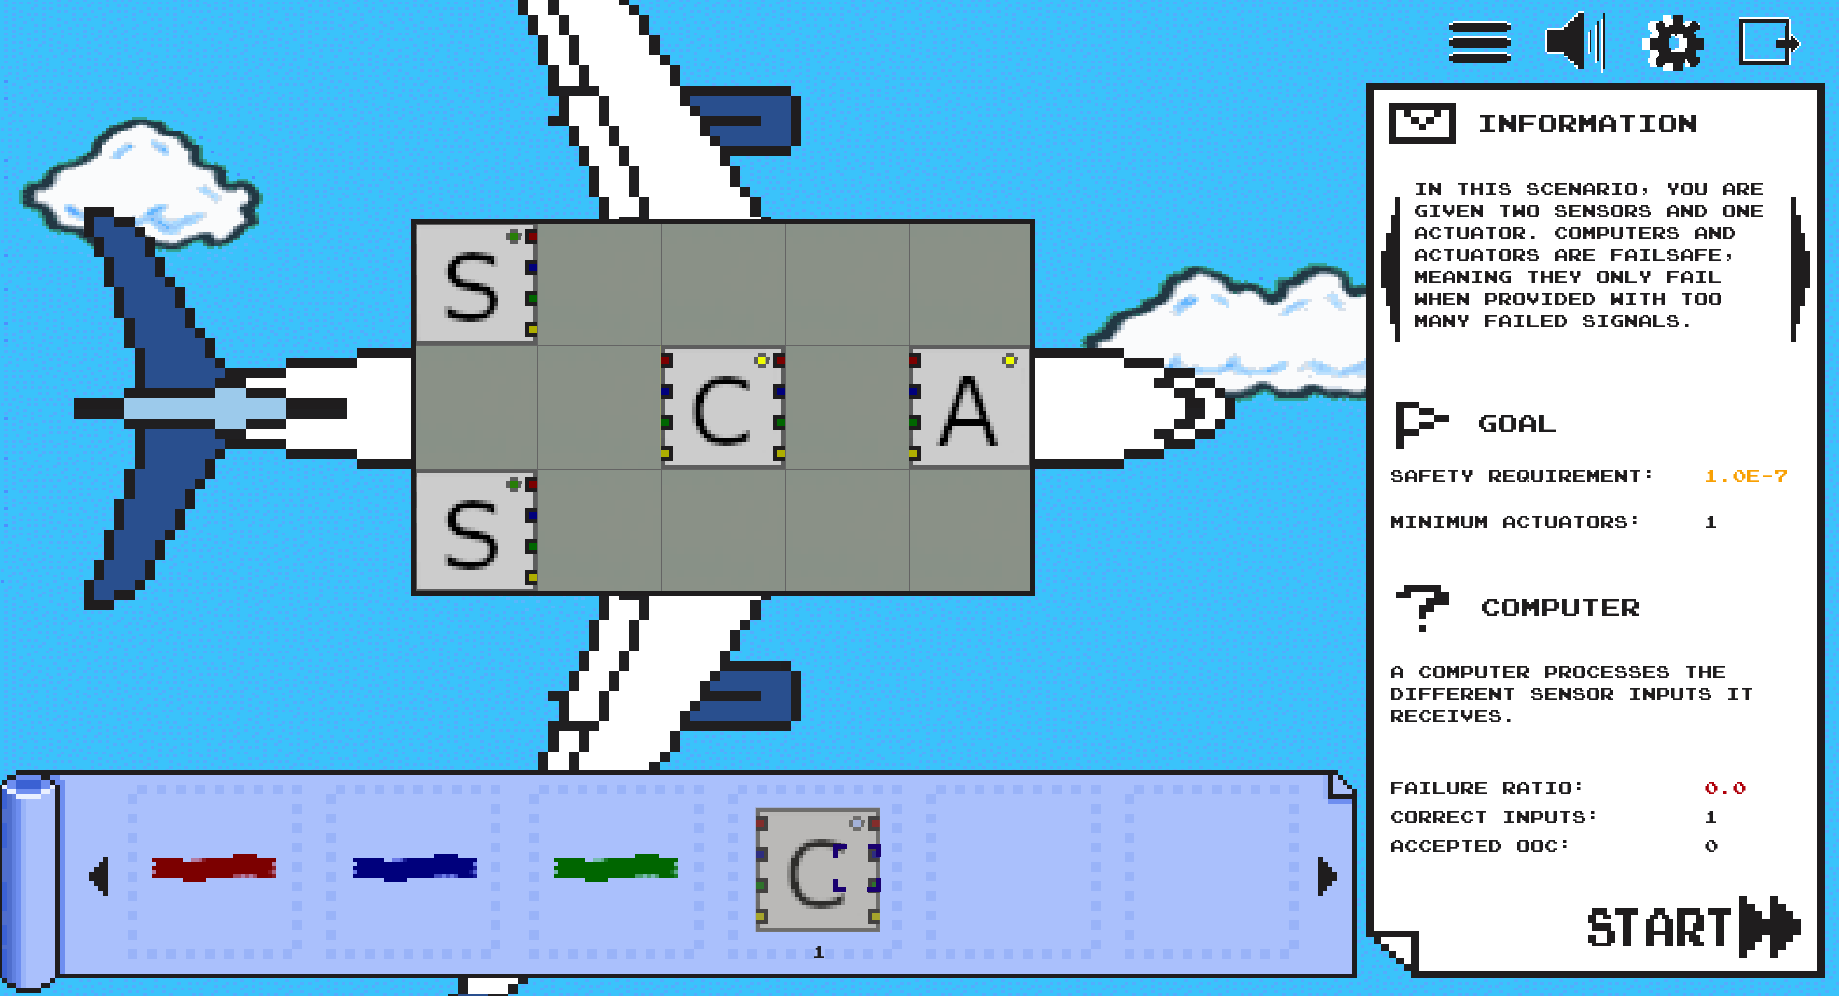
\includegraphics[width=0.9\textwidth]{Pictures/res/implementation/scenes/game-scene}
    }
    \caption{Game Scene}
    \label{fig:game-scene}
\end{figure}

\begin{figure}
    \centering
    \setlength{\fboxsep}{1pt}
    \setlength{\fboxrule}{1pt}
    \fbox{
        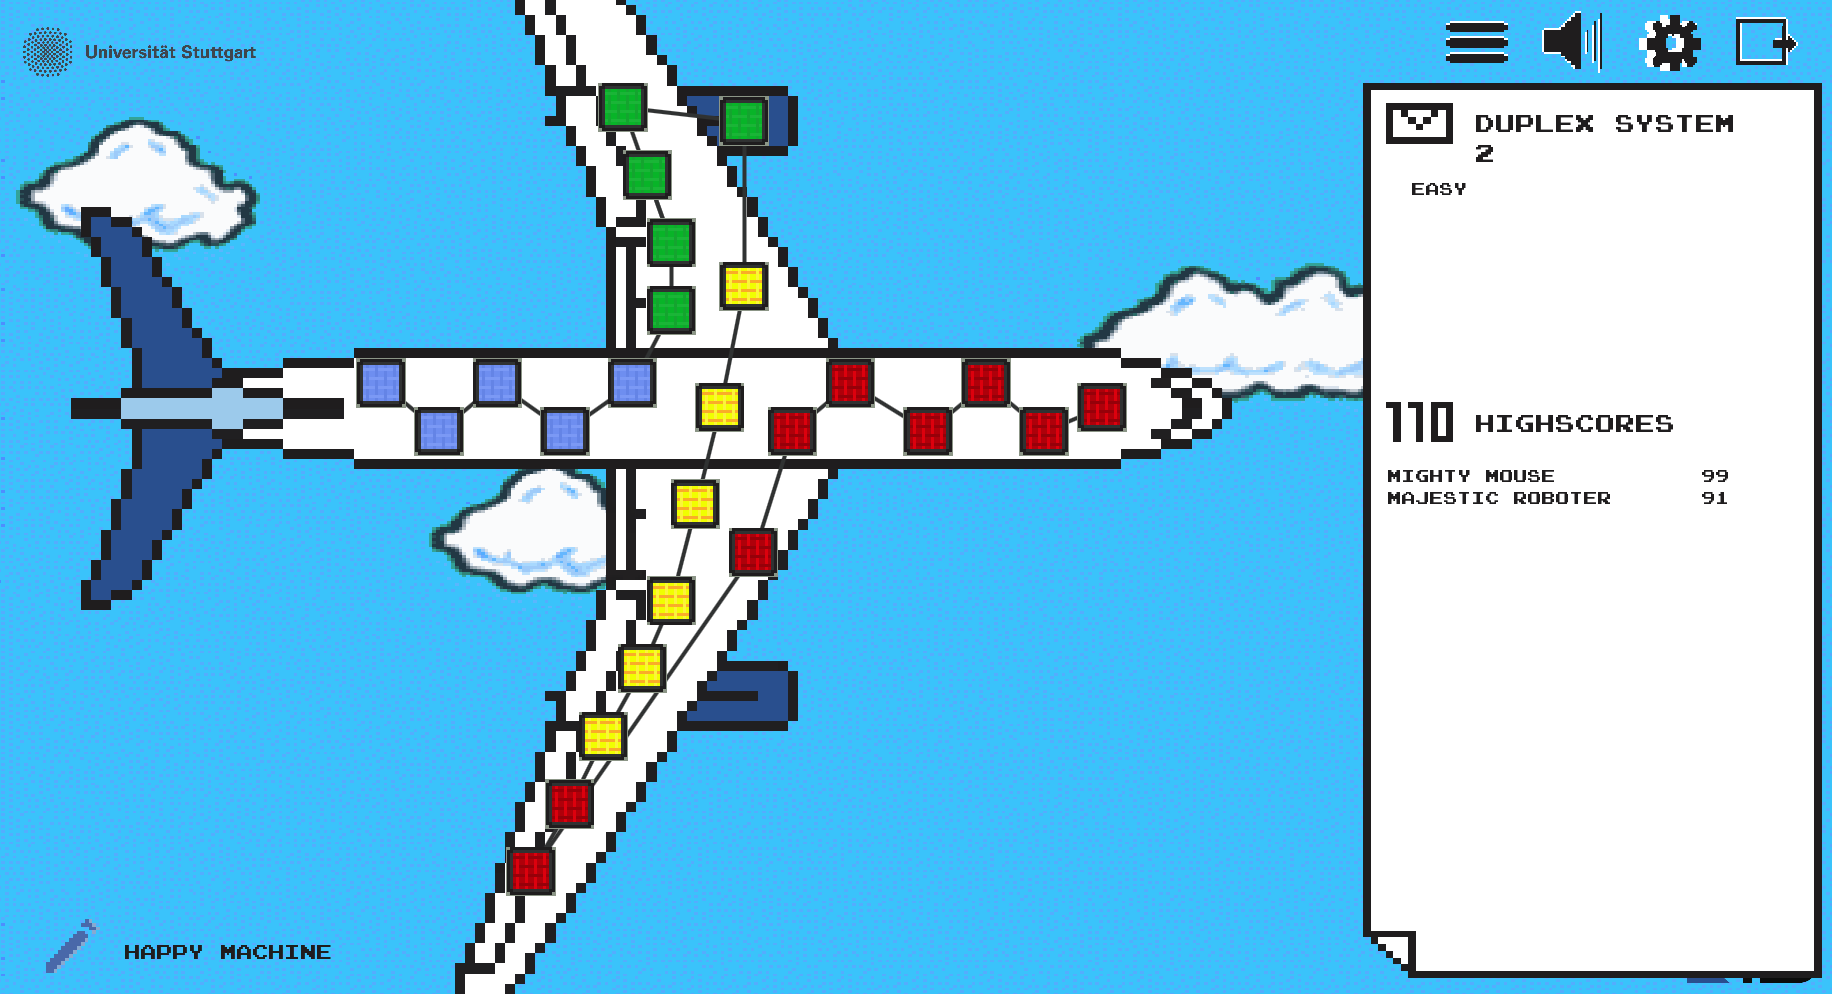
\includegraphics[width=0.9\textwidth]{Pictures/res/implementation/scenes/level-map}
    }
    \caption{Level Map Scene}
    \label{fig:level-scene}
\end{figure}

\begin{figure}
    \centering
    \setlength{\fboxsep}{1pt}
    \setlength{\fboxrule}{1pt}
    \fbox{
        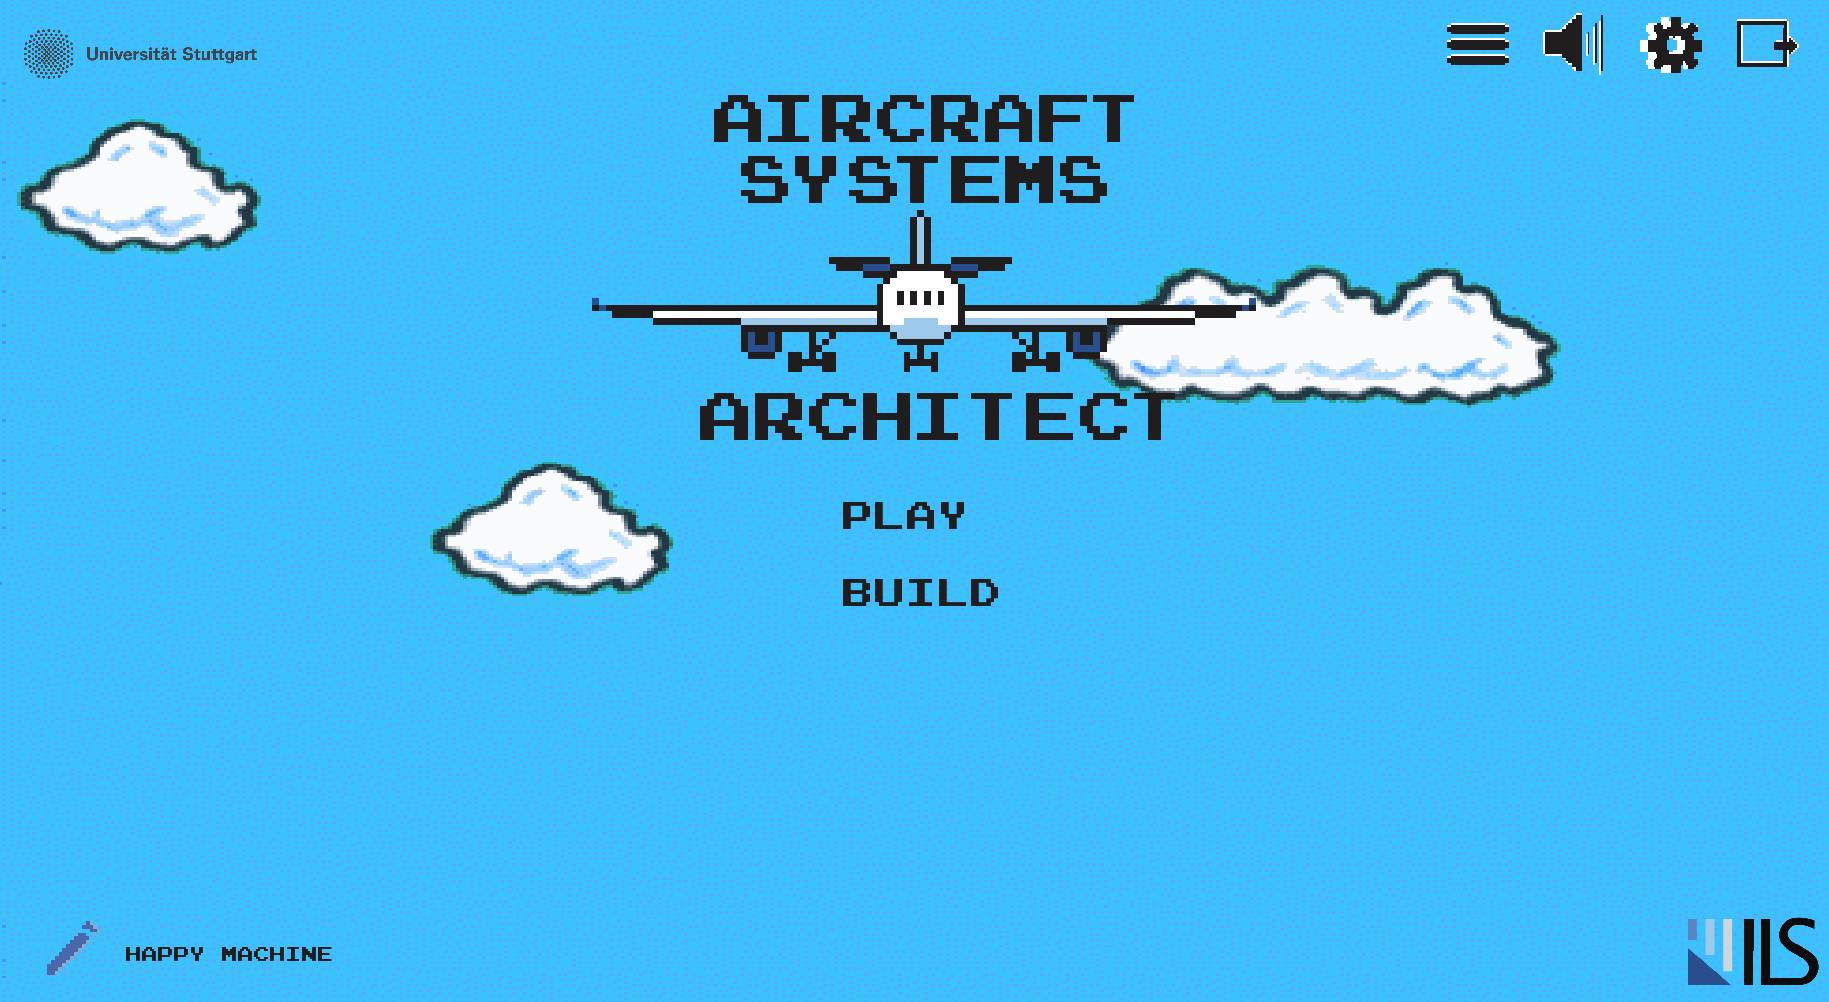
\includegraphics[width=0.9\textwidth]{Pictures/res/implementation/scenes/main-menu}
    }
    \caption{Menu Scene}
    \label{fig:menu-scene}
\end{figure}

\subsubsection{Entities}
\textbf{Grid Entities:} \\
Grid entities describe each tile of the grid, containing a grid position as $(x,y)$ coordinates and a customizable grid tile,
which is usually the regular concrete background, but may be changed any time for specific scenarios.

\textbf{Simulation Entities:} \\
All elements that are placed on the game grid are considered so-called Simulation Entities.
These entities are built of components to describe the cable port distribution, parameters such as failure ratio and failure detection ratio and grid components, which contain the
entities position as a coordinate in the games' grid-like game field.
Each entity that should have a description on the right side tool box also has a TooltipComponent attached, which indicates, that
a tooltip should be shown when hovering the entity.
Furthermore, graphics and colliders are available to simulation entity objects.
\\
\textbf{Build Panel Entities:} \\
Build Panel Entities are entities which are available in the players' inventory and can be used for building objects on the game grid.
They include components for graphics description, build information - e.g.\ the failure ratio, failure detection ratio and amount in inventory,
and colliders.
Similar to the simulation entity, a tooltip component is also available to the build panel entities to indicate tooltip descriptions.
\\

\subsubsection{Components}
The above-mentioned entities implement different components to store the according data and to identify which component
should implement certain behaviors such as being able to be built to the grid or adding them to the simulation.
The following components were developed and implemented during the game development process.
\\
\textbf{GridComponent:} \\
The GridComponent stores the grid position as $(x,y)$ coordinates of an entity, where $x=0, y=0$ is the top left of the game grid.
\\
\textbf{SimulationComponent:} \\
Data regarding the simulation run by the MarkovProcessor is stored in the SimulationComponent.
The simulation type (i.e. Actuator, Sensor, Computer, \ldots), as well as the current state (i.e. inoperative, correct by default, ...), failure
ratio and failure detection ratio are stored.
Furthermore, the component contains parameters to store the entity ids of entities connected as inputs to this component / entity, which is
not necessary, however enables easier maintainable code and performant look-ups for some systems.
\\
\textbf{BuildComponent:} \\
The BuildComponent is used to tell the systems operating the game, that an entity should be buildable.
Therefore, it contains similar information as the simulation component, as the parameters from the build component are used
to create new simulation entities with simulation components attached when placing a component on the grid.
Furthermore, the build component also stores the amount of components on the stack.
As this number would go below 0, no new component can be built.

\\
\textbf{CablePortsComponent:} \\
CablePortsComponents contain data regarding the connection of entities to each other.
Each CablePortComponent can have multiple in- or outgoing cable ports.
Cable ports are used to store another entity object, which describes the entity connect to another entity.
When updating a connection, both sides of the connection have to be considered.
A cable ports' connected entity parameter may be null, when there is currently no connection to the port.

\\
\textbf{ToolTipComponent:} \\
The tooltip component may be used for entities that should display a tooltip upon hovering over the object with the cursor.
Information such as failure ratio, simulation type and description of the object are stored as text strings (as ids, which are read
from the language file, or as converted numbers to strings) in this component, so they may be directly used to render them to
the screen.
\subsubsection{Entity UML}
A comprehensive overview of the different entity structures is given in~\ref{fig:entities}.
\begin{figure}
    \centering
    \includegraphics[width=\textwidth]{Pictures/res/implementation/entities-uml}
    \caption{UML Diagrams of the different entities}
    \label{fig:entities}
\end{figure}
\todo{create uml}

\subsection{Level Implementation}\label{subsec:level-implementation}
Each level is created as a new GameScene object with the content of a level file that is read and parsed by the resource
manager~\ref{sec:data-storage-&-data-parsing}.
The GameScene object stores all relevant data, including the level requirements / goal, the grid size, available entities and, if applicable through the
tutorial interface implementation, possible dialogues and character models that form the tutorial scene.
Following examples for different levels are provided in this chapter:
\begin{itemize}
    \item Tutorial Scene explaining the basics of the gameplay~\ref{fig:basic-gameplay-tutorial}
    \item Duplex System~\ref{fig:duplex-system}
    \item Common-Mode Scenario, with different types of sensors and computers~\ref{fig:common-mode-scene}
    \item Oil leakage scenario, emulating a common-cause failures~\ref{fig:common-cause-scene}
\end{itemize}
\todo{add scene pictures}
\begin{figure}
    \centering
    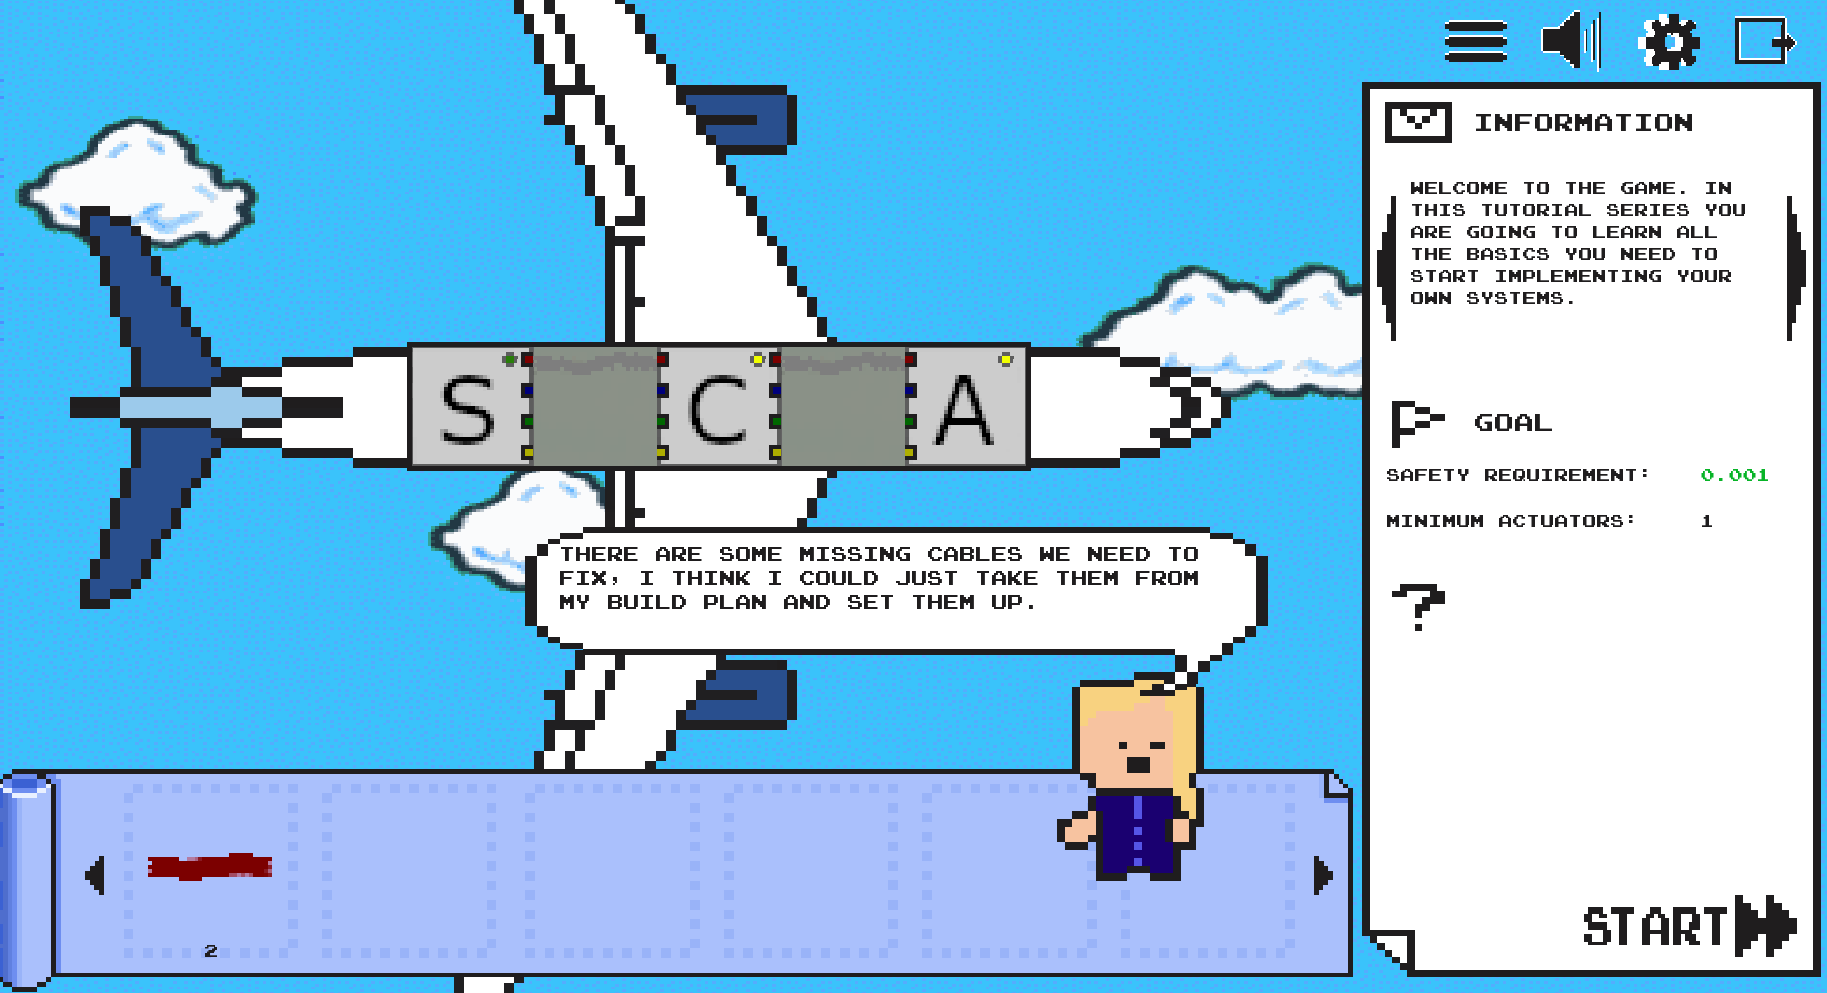
\includegraphics[width=\textwidth]{Pictures/res/implementation/scenes/tutorial-game-scene}
    \caption{Tutorial Scene with dialogue to explain basic gameplay}
    \label{fig:basic-gameplay-tutorial}
\end{figure}
\begin{figure}
    \centering
    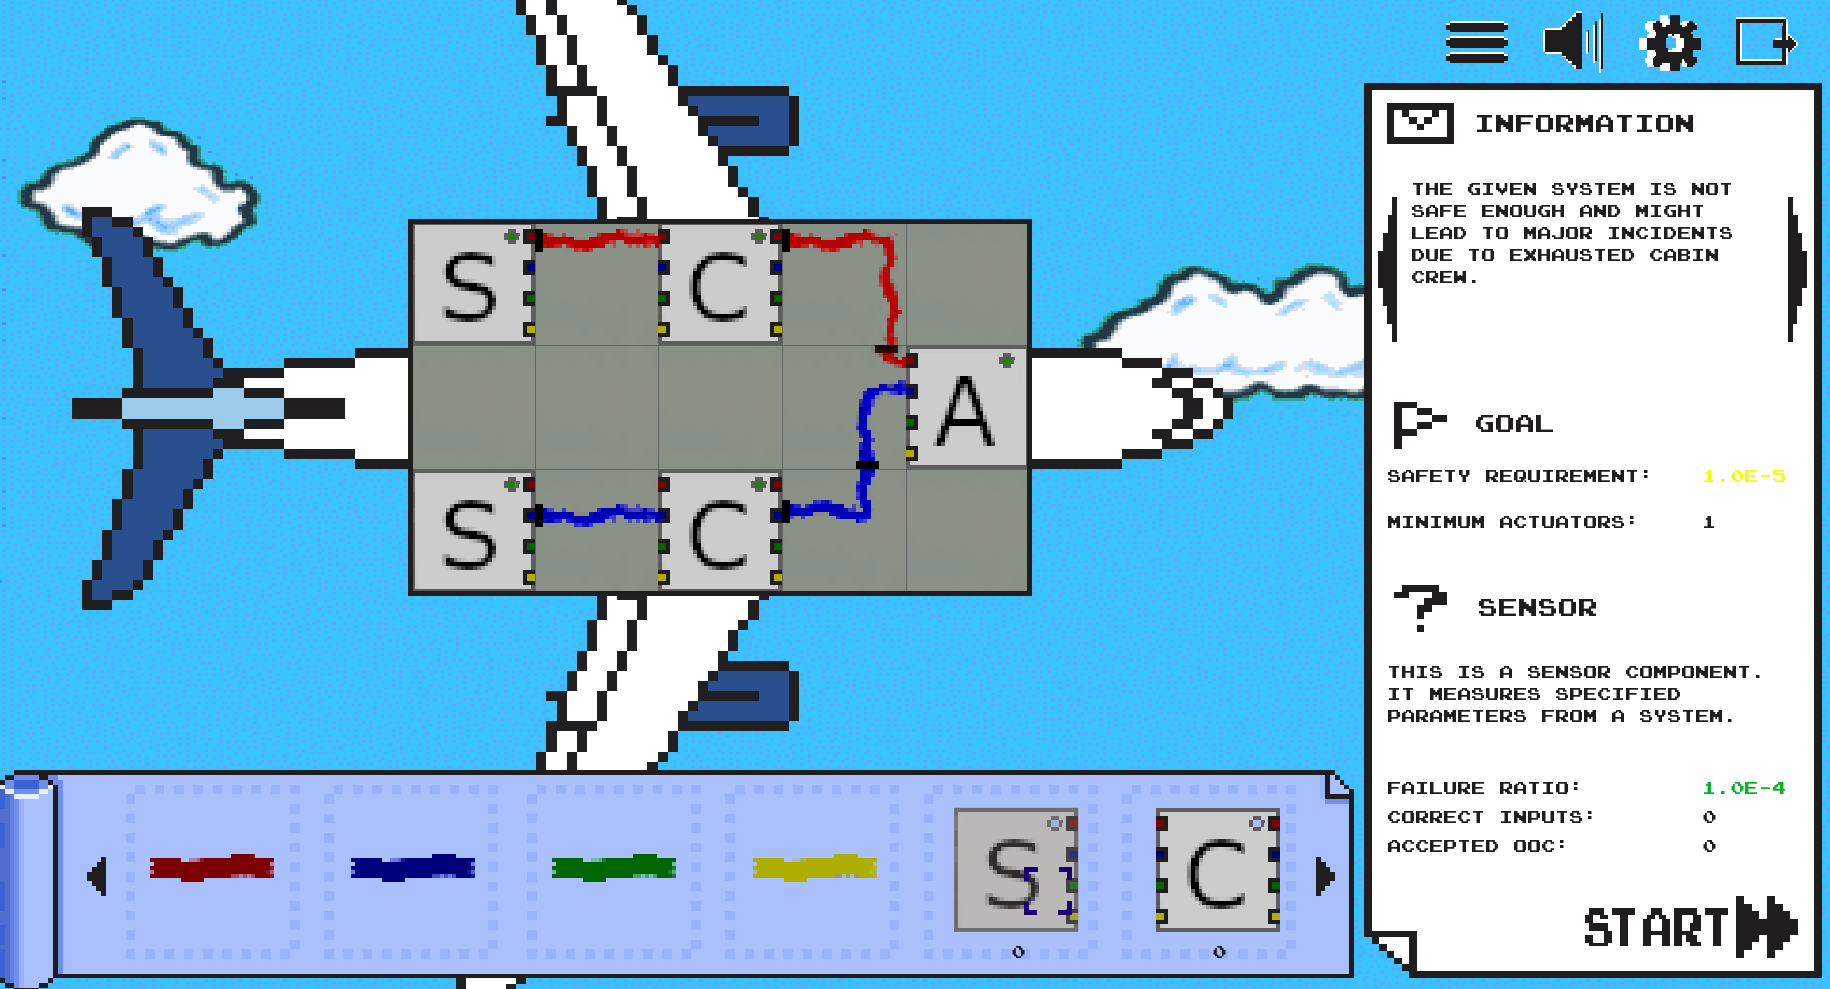
\includegraphics[width=\textwidth]{Pictures/res/implementation/scenes/duplex-scene}
    \caption{Scenario to set up a duplex system}
    \label{fig:duplex-system}
\end{figure}
\begin{figure}
    \centering
    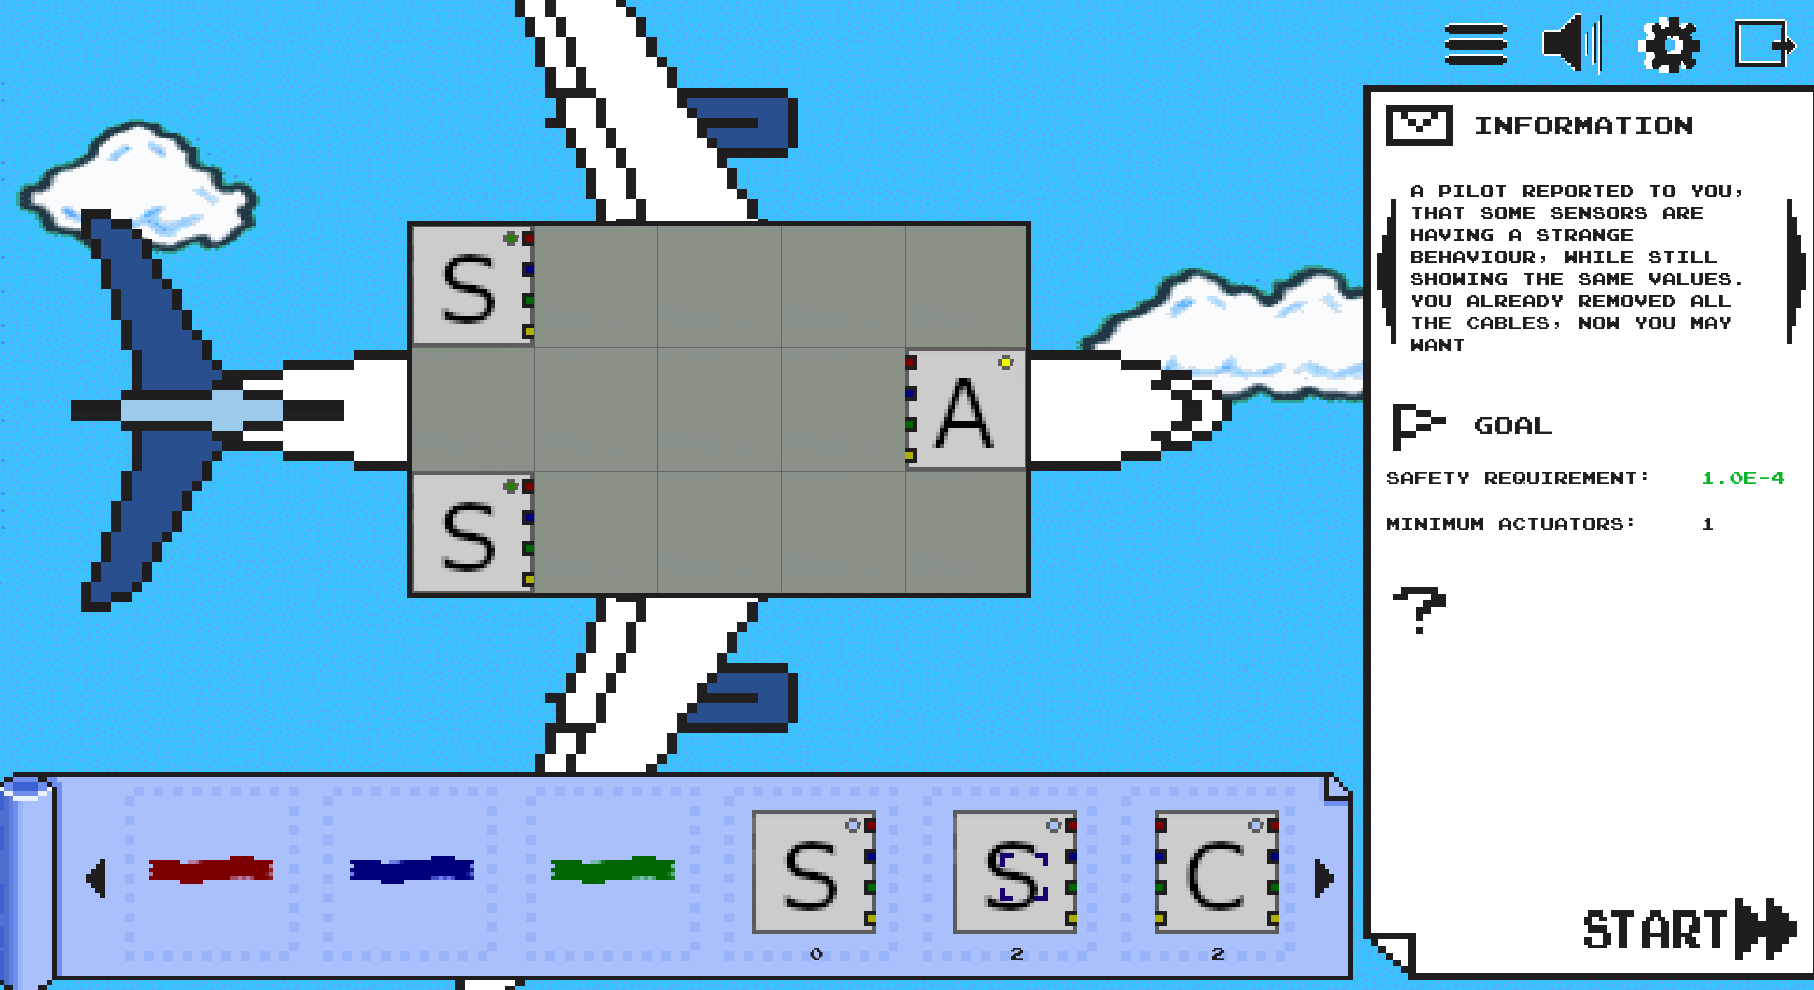
\includegraphics[width=\textwidth]{Pictures/res/implementation/scenes/cmf}
    \caption{Multiple useable sensors to visualize common mode failures}
    \label{fig:common-mode-scene}
\end{figure}
\begin{figure}
    \centering
    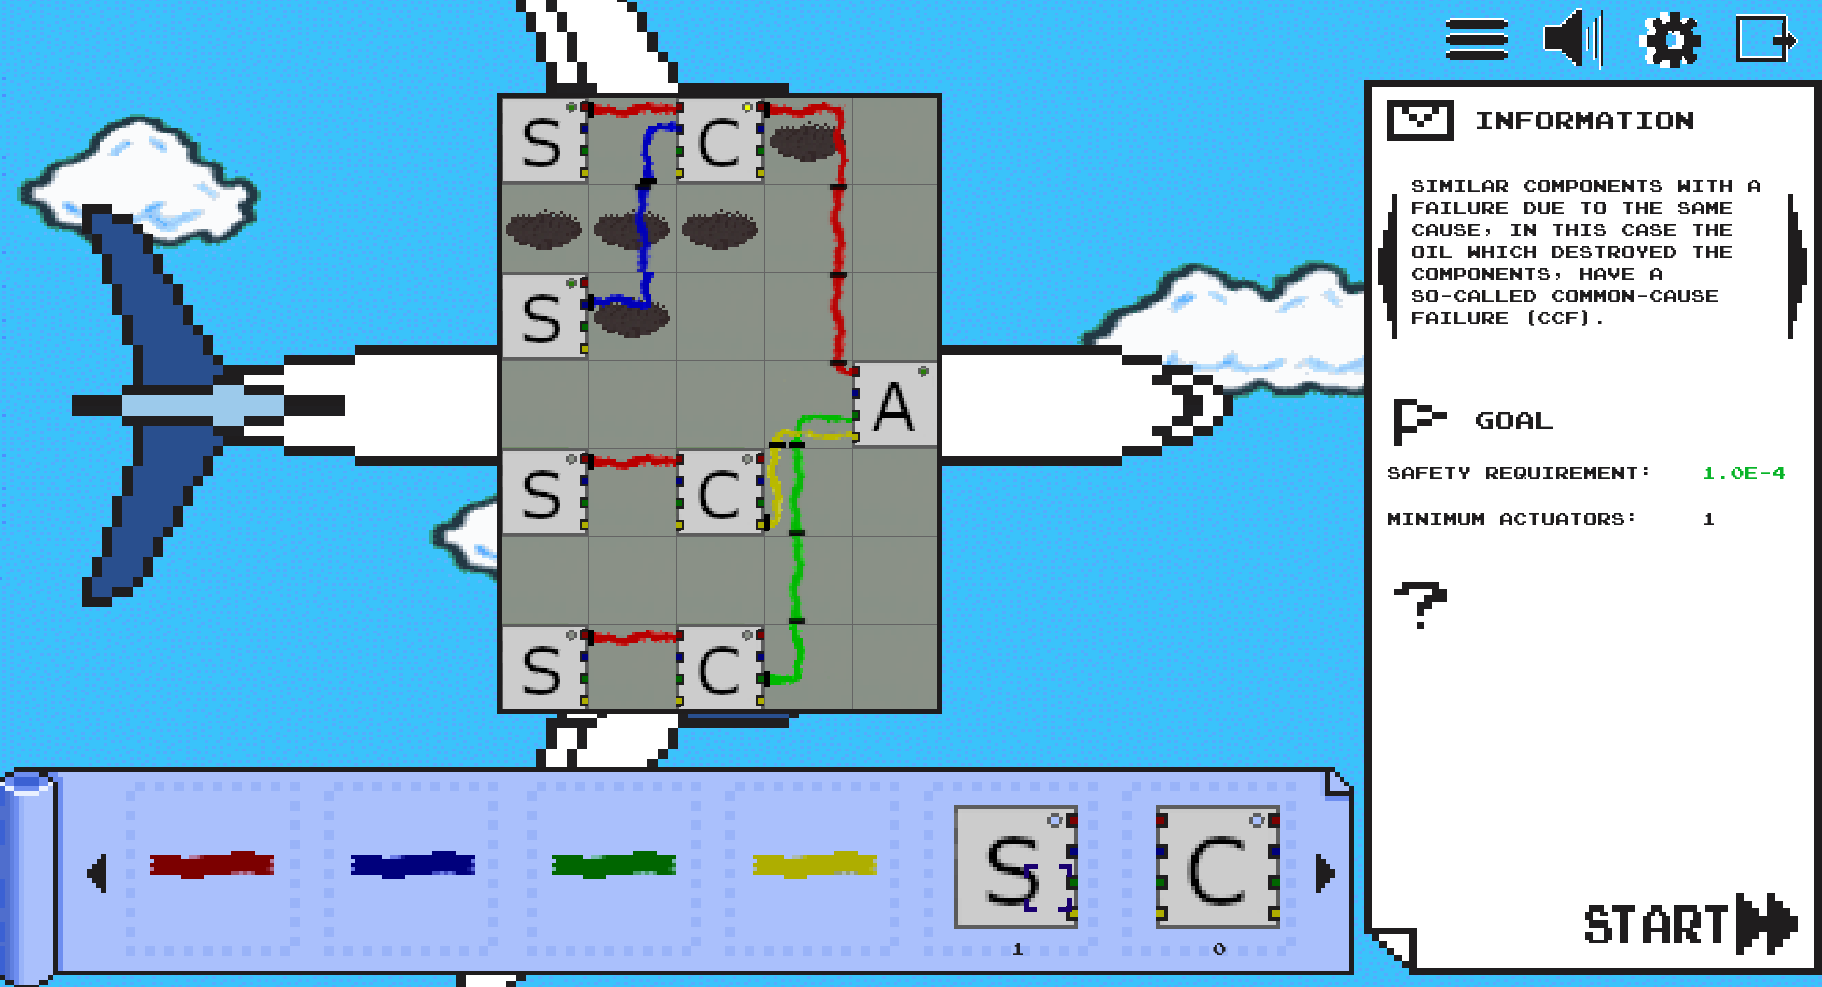
\includegraphics[width=\textwidth]{Pictures/res/implementation/scenes/oil-leak}
    \caption{A scene with an oil leakage on one side of the system to visualize common cause failures}
    \label{fig:common-cause-scene}
\end{figure}

For the game grid, tile sets as explained in \ref{subsec:tileset} are used, which consist of different images for different components.
Figure~\ref{fig:tileset} shows all tiles that are currently available to the game implementation.
This is easily extendable by adding more tiles to the set, which may be used for backgrounds, placeholders or new simulation entities.
\begin{figure}
    \centering
    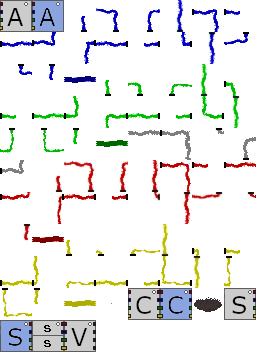
\includegraphics[width=\textwidth]{Pictures/res/implementation/tileset}
    \caption{Tileset}
    \label{fig:tileset}
\end{figure}

\subsubsection{Tutorial Scenes}\label{subsubsec:tutorial-scenes}
In order to explain the gameplay, tutorial dialogues were implemented to some scenes of the game.
To make the dialogues interesting and appealing, characters were designed to make the tutorials engaging and interactive.
In figure~\ref{fig:character-models} the character models used in the implementation are shown.
This is easily extendable and more characters may be added to the game to create more tutorials or other dialogues and maybe even create
a story in the future, that uses the character designs.
\begin{figure}
    \centering
    
\includegraphics[width=\textwidth]{Pictures/res/implementation/character-models}
    \caption{Character Models (left to right): Tina Technician, Ingo Engineer, Pete Pilot}
    \label{fig:character-models}
\end{figure}

\section{Data Storage \& Data Parsing}\label{sec:data-storage-&-data-parsing}
It was chosen to save and load resources from XML files, due to the benefits of this file format.
XML stands for eXtensible Markup Language, and it is a markup language that is used for encoding documents in a format that is both human-readable and machine-readable.
It was designed to be flexible and extensible, allowing developers to create their own markup tags and structure data in a way that is specific to their needs.
\\
XML documents are made up of elements, which are enclosed in opening and closing tags, and attributes, which provide additional information about the element.
The structure of an XML document is defined by a Document Type Definition (DTD) or an XML Schema, which specifies the elements and attributes that are allowed in the document and the relationships between them.
\\
One of the main benefits of XML is its ability to store and transfer data in a standardized format that can be easily parsed by different software applications, regardless of the platform, and there are
already multiple implementations available to successfully do this, including JAVA's built-in library for DOM parsing.
\\
The structure of the different XML files for levels, tilesets, scores and language used in this project will be explained in the next chapters.
\subsection{Tileset}\label{subsec:tileset}
A tileset file contains a list of multiple tile nodes, which each have an id and a type attribute.
A tile always contains exactly one image node, which has at least width, height and a resource path to an image assigned to it.
Optionally, there can also be a description attribute which can be used to set a tooltip that will be rendered to the games tooltip panel, if available.
\\
The following example shows a tileset with a single tile of the type CPU, including its description and image parameters.
\\ \\
\begin{lstlisting}[language=XML,label={lst:tileset-xml}]
    <?xml version="1.0" encoding="UTF-8"?>
    <tileset name="tiles">
        <tile id="200" type="CPU">
            <image width="32" height="32" source="res/avionics/default.png" description="Default CPU Component"/>
        </tile>
    </tileset>
\end{lstlisting}
\subsection{Level Files}\label{subsec:level-files}
The root node of a level structure is the map node, which always contains attributes to assign an id, a name, a difficulty (tutorial, easy, medium, hard or custom) and a
grid width and height for the games grid.
The map node contains one sub node for descriptions (and description parts, if the text for a description should be split up into multiple displayable parts),
one sub node for available elements to build from the build panel and one sub node that defines the already available objects on the grid.
Additionally, the goal and goal definition sub nodes contain information on how to pass a level (i.e.\ safety requirement, minimum components that should be working correctly and
maximum ouf of control components).
Furthermore, the tileset used by this map needs to be defined in the tileset sub node and unlocks (i.e.\ which level ids are unlocked after passing this level) can be defined.
\\
The below code shows an example on the structure of the level xml files, which describes a 5 by 3 game grid with one actuator
at position $x = 4$ and $y = 1$, and two sensors at positions $x = 0$ and $y = [0, 2]$.
\\
Note, that the width and height attributes represent the actual size of the map, similar to the length of an array in Java, while
the positions show the position in the grid starting at 0, similar to indexes in Java arrays.
\\
\\
\begin{lstlisting}[language=XML,label={lst:level-xml}]
    <?xml version="1.0" encoding="UTF-8"?>
    <map id="0" name="@0" width="5" height="3" difficulty="EASY">
        <description>
            <part>@1</part>
        </description>
        <goal>1e-7</goal>
        <goalDefinition workingActuators="1" workingSensors="0" workingComputers="0"/>
        <tileset source="base_tiles.xml"/>
        <unlocks>
            <unlock>6</unlock>
        </unlocks>
        <build>
            <entity id="500" amount="1000" safety="0" correctSignalsNeeded="1" outOfControlSignalsAccepted="0"/>
            <entity id="501" amount="1000" safety="0" correctSignalsNeeded="1" outOfControlSignalsAccepted="0"/>
            <entity id="502" amount="1000" safety="0" correctSignalsNeeded="1" outOfControlSignalsAccepted="0"/>
            <entity id="203" amount="2" safety="0" failureDetectionRatio="1" correctSignalsNeeded="1"
                    outOfControlSignalsAccepted="0"/>
        </build>
        <layer id="0" name="Tile Layer 1">
            <entity x="0" y="0" id="201" interactable="false" safety="1e-4" failureDetectionRatio="1"
                    correctSignalsNeeded="0" outOfControlSignalsAccepted="0"/>
            <entity x="0" y="2" id="201" interactable="false" safety="1e-4" failureDetectionRatio="1"
                    correctSignalsNeeded="0" outOfControlSignalsAccepted="0"/>
            <entity x="4" y="1" id="205" interactable="false" safety="0" failureDetectionRatio="1" correctSignalsNeeded="2"
                    outOfControlSignalsAccepted="0"/>
        </layer>
    </map>
\end{lstlisting}
\subsection{Language Files}\label{subsec:language-files}
A language file contains all text content used in the game for a specified language.
In the root node, the language type can be given according to the IETF language tag \todo{add source}, if supported by the game (i.e.\ implemented in the language manager).
Within this root node, string nodes are created which contain the id of a string as an attribute and the actual content as text.
Each of the ids has to be unique, otherwise only the first specified id will be considered in the implementation.
\\
\\
\begin{lstlisting}[language=XML,label={lst:lang-xml}]
    <strings language="">
        <string id="1">Sample Text</string>
    </strings>
\end{lstlisting}

\subsection{Score Files}\label{subsec:score-files}
Highscores for each level are saved in a separate xml file containing information about the profile name, score and level id.
The following structure is used for this file, saving the score 91 for a user who played level id one.
\\ \\
\begin{lstlisting}[language=XML,label={lst:score-xml}]
    <scores>
      <scoreItem>
        <name>User</name>
        <score>91</score>
        <level>1</level>
      </scoreItem>
    </scores>
\end{lstlisting}

\subsection{Parsing}\label{subsec:parsing}
For data parsing, a standard DOM parser library provided by Java is used.
It handles all possible exception types, such as input exceptions or malformed xml documents by default and allows for a quick setup of parsing
the necessary nodes, attributes and text contents from the given input files.
As each type of file handled by default for this game has a different structure, the ResourceManager and its sub managers implement methods to handle
each file structure: loading a level, loading a tileset, loading scores, loading language data and loading fonts.

\section{External Device Inputs}\label{sec:external-device-inputs}
As the game developed in this work will mostly be played by a younger age group, an additional requirement was to play this game not only by mouse and keyboard,
but also by gamepads.
The reason being, that with a gamepad, there will be more of a game-like environment provided to the users.
The integration of gamepads such as game controllers is explained in this chapter.
\subsection{Mouse \& Keyboard}\label{subsec:mouse-&-keyboard}
The standard input device for the game are mouse and keyboard.
\subsection{Gamepad Integration}\label{subsec:gamepad-integration}
The game was designed for was keyboard and mouse, however due to the easy accessibility requirement, it was chosen to also implement gamepad integration.
For gamepad integration, the open source library \textit{Jamepad} is used.
It automatically detects most USB controller devices and has an inbuilt button mapping which can be used in the implementation.
A separate thread with a capture rate for controls which is equal and synchronized to the games' FPS is implemented to queue all controller
events to the game engines' event queue and action system, where they are handled.
Button handling is mostly implemented in a way that a button press creates a new mouse event and the cursor position which is then handled by the action
systems' mouse event handling method.
This reduces maintenance and new implementation of buttons and actions, while being guaranteed to work correctly with all devices.


